% This template was originally by R. Jacob Vogelstein
% Updated on March 1, 2010 by Noah J. Cowan
% Updated on May 18, 2014 by Brian Weitzner at https://github.com/weitzner/jhu-thesis-template
% Updated on January 29, 2016 by John Muschelli at https://github.com/muschellij2/PhD_Thesis
% Updated on April 13, 2016 by Leonardo Collado Torres and available at https://github.com/lcolladotor/jhu-thesis-template. View (read-only) at Overleaf here https://www.overleaf.com/read/tqdzgmrxgbtg

%% It's your responsability to make sure that your thesis complies with 
%% JHU's formatting rules available at http://guides.library.jhu.edu/etd/formatting

\documentclass[12pt]{report}

%% This was the setup recommended at https://github.com/weitzner/jhu-thesis-template
% \documentclass[12pt,oneside,final]{thesis}

\pdfminorversion=4\relax
\pdfobjcompresslevel=0\relax
%% Followed the information from https://www.overleaf.com/latex/examples/creating-pdf-slash-a-and-pdf-slash-x-files/bbbycnbyqhnm#.Vw6_XBMrLm1 to create a PDF/A file in Overleaf
\usepackage[a-1b]{pdfx} % Need this to create a PDF/A file

\usepackage{pdfpages}

\pagestyle{myheadings}
%\topmargin=0.25in
\topmargin=0.05in
\textheight=8.15in
\textwidth=5.6in
\oddsidemargin=0.7in
\raggedbottom
\newdimen \jot \jot=5mm
\brokenpenalty=10000
 
 % Settings for debugging
%\tracinggroups=1
%\tracingnesting=2

% standalone package, "simplifies" compilations of multi-source document
%\usepackage{standalone}

% custom packages
\usepackage{sty/er-abbrev}
\usepackage{sty/er-math}
\usepackage{sty/er-paper}
\usepackage{sty/mk-outline}
\usepackage{sty/mk-chem-notation}
\usepackage{sty/mk-ffpilot-notation}
\usepackage{sty/mk-stats-notation}

% some geometry setting stuff. Useful if not done elsewhere
%\usepackage[top=0.85in,left=0.75in,footskip=0.75in]{geometry}

% for bib file and bibliography support
%\usepackage[numbers,sort&compress]{natbib}

%\usepackage{amsmath,amssymb}
%\usepackage{mathtools}

% Use Unicode characters when possible
%\usepackage[utf8]{inputenc}

% for acronyms
%\usepackage[nolist]{acronym}

% line numbers
\usepackage[right]{lineno}

% don't remember what this is for
\usepackage{calc}

% Load any custom macros or abbreviations from abbreviations.tex
% Abbreviations and command definitions.
\defineAbbreviation{CA}{cellular automata}
\defineAbbreviation{CET}{cryoelectron tomography}
\defineAbbreviation{CME}{chemical master equation}
\defineAbbreviation{CPU}{central processing unit}
\defineAbbreviation{CUDA}{Compute Unified Device Architecture}
\defineAbbreviation{DGL}{differential gene loss}
\defineAbbreviation{DS}{direct sampling}
\defineAbbreviation{ds-protein}{domain specific ribosomal protein}
\defineAbbreviationPlural{ds-protein}{ds-proteins}{domain specific ribosomal proteins}
\defineAbbreviation{EF-Tu}{elongation factor Tu}
\defineAbbreviation{EN}{extrinsic noise}
\defineAbbreviation{EP}{evolutionary profile}
\defineAbbreviation{ERM}{equal-rates Markov}
\defineAbbreviation{ES}{enhanced sampling}
\defineAbbreviation{FBA}{flux balance analysis}
\defineAbbreviation{FFPilot}{forward flux pilot sampling}
\defineAbbreviation{FPE}{Fokker-Planck equation}
\defineAbbreviation{GFP}{green fluorescent protein}
\defineAbbreviation{GPU}{graphics processing unit}
\defineAbbreviationPlural{GPU}{GPUs}{graphics processing units}
\defineAbbreviation{GRF}{gene regulation function}
\defineAbbreviation{GMP}{Gillespie multi-particle}
\defineAbbreviation{GTS}{genetic toggle switch}
\defineAbbreviation{HDFS}{Hadoop distributed file system}
\defineAbbreviation{HGT}{horizontal gene transfer}
\defineAbbreviation{HPC}{high performance computing}
\defineAbbreviation{IN}{intrinsic noise}
\defineAbbreviation{indel}{insertion or deletion}
\defineAbbreviationPlural{indel}{indels}{insertions or deletions}
\defineAbbreviation{IPTG}{isopropyl $\beta$-D-1-thiogalactopyranoside}
\defineAbbreviation{KL}{Kullback--Leibler}
\defineAbbreviation{LacI}{{\it lac} repressor}
\defineAbbreviation{LacY}{lactose permease}
\defineAbbreviation{LMES}{Lattice Microbes ES} 
\defineAbbreviation{LSU}{large subunit}
\defineAbbreviation{ME-EP}{maximum-entropy evolutionary profile}
\defineAbbreviation{MD}{molecular dynamics}
\defineAbbreviation{MFPT}{mean first passage time}
\defineAbbreviation{ML}{maximum-likelihood}
\defineAbbreviation{MPD}{mulitparticle diffusion}
\defineAbbreviation{MPD-RDME}{mulitparticle-diffusion RDME}
\defineAbbreviation{MR-RDME}{multiresolution RDME}
\defineAbbreviation{mRNA}{messenger RNA}
\defineAbbreviation{MSA}{multiple sequence alignment}
\defineAbbreviation{MSD}{mean square displacement}
\defineAbbreviation{MST}{mean switching time}
\defineAbbreviationPlural{MST}{MSTs}{mean switching times}
\defineAbbreviation{nm}{nanometers}
\defineAbbreviation{ns}{nanoseconds}
\defineAbbreviation{ODE}{ordinary differential equation}
\defineAbbreviationPlural{ODE}{ODEs}{ordinary differential equations}
\defineAbbreviation{OU}{Ornstein-Uhlenbeck}
\defineAbbreviation{PDE}{partial differential equation}
\defineAbbreviationPlural{PDE}{PDEs}{partial differential equations}
\defineAbbreviation{PDF}{probability density function}
\defineAbbreviationPlural{PDF}{PDFs}{probability density functions}
\defineAbbreviation{PFB}{positive feedback}
\defineAbbreviation{QBIO}{quantitative biology}
\defineAbbreviation{RBS}{ribosomal binding site}
\defineAbbreviation{RMSD}{root-mean-square deviation}
\defineAbbreviation{RNAP}{RNA polymerase}
\defineAbbreviation{REU}{Research Experiences for Undergraduates}
\defineAbbreviation{RDME}{reaction-diffusion master equation}
\defineAbbreviation{rRNA}{ribosomal RNA}
\defineAbbreviation{r-protein}{ribosomal protein}
\defineAbbreviationPlural{r-protein}{r-proteins}{ribosomal proteins}
\defineAbbreviation{SCT}{single-cell trap}
\defineAbbreviation{SSA}{stochastic simulation algorithm}
\defineAbbreviation{SSU}{small subunit}
\defineAbbreviation{SI}{supporting information}
\defineAbbreviation{SOQ}{Summer of QBIO}
\defineAbbreviation{SRG}{self-regulating gene}
\defineAbbreviation{SRP}{signal recognition particle}
\defineAbbreviation{TMG}{thiomethyl-$\beta$-D-galactoside}
\defineAbbreviation{TRN}{transcriptional regulatory network}
\defineAbbreviation{TOC}{table of contents}
\defineAbbreviation{UPT}{universal phylogenetic tree}
\defineAbbreviation{VM}{virtual machine}

% Species abbreviations.
\defineAbbreviationStrict{Ametal}{\textit{A. metalliredigens}}{\textit{Alkaliphilus metalliredigens}}
\defineAbbreviationStrict{Aorem}{\textit{A. oremlandii}}{\textit{Alkaliphilus oremlandii}}
\defineAbbreviationStrict{Bsubt}{\textit{B. subtilis}}{\textit{Bacillus subtilis}}
\defineAbbreviationStrict{Cacet}{\textit{C. acetobutylicum}}{\textit{Clostridium acetobutylicum}}
\defineAbbreviationStrict{Celegans}{\textit{C. elegans}}{\textit{Caenorhabditis elegans}}
\defineAbbreviationStrict{Cnovyi}{\textit{C. novyi}}{\textit{Clostridium novyi}}
\defineAbbreviationStrict{Dradio}{\textit{D. radiodurans}}{\textit{Deinococcus radiodurans}}
\defineAbbreviationStrict{Ecoli}{\textit{E. coli}}{\textit{Escherichia coli}}
\defineAbbreviationStrict{Fmagna}{\textit{F. magna}}{\textit{Finegoldia magna}}
\defineAbbreviationStrict{Hmaris}{\textit{H. marismortui}}{\textit{Haloarcula marismortui}}
\defineAbbreviationStrict{Lborg}{\textit{L. borgpetersenii}}{\textit{Leptospira borgpetersenii}}
\defineAbbreviationStrict{Mflag}{\textit{M. flagellatus}}{\textit{Methylobacillus flagellatus}}
\defineAbbreviationStrict{Mtuber}{\textit{M. tuberculosis}}{\textit{Mycobacterium tuberculosis}}
\defineAbbreviationStrict{Pingr}{\textit{P. ingrahamii}}{\textit{Psychromonas ingrahamii}}
\defineAbbreviationStrict{Saren}{\textit{S.  arenicola}}{\textit{Salinispora  arenicola}}
\defineAbbreviationStrict{Scerev}{\textit{S. cerevisiae}}{\textit{Saccharomyces cerevisiae}}
\defineAbbreviationStrict{Scoel}{\textit{S. coelicolor}}{\textit{Streptomyces coelicolor}}
\defineAbbreviationStrict{Ssolf}{\textit{S. solfataricus}}{\textit{Sulfolobus solfataricus}}
\defineAbbreviationStrict{Strop}{\textit{S. tropica}}{\textit{Salinispora tropica}}
\defineAbbreviationStrict{Ttherm}{\textit{T. thermophilus}}{\textit{Thermus thermophilus}}

% Grammar shortcuts.
\newcommand{\ie}{\textit{i.e.}\xspace}
\newcommand{\eg}{\textit{e.g.}\xspace}
\newcommand{\etal}{\textit{et al.}\xspace}

% Biology shortcuts.
\newcommand{\insitu}{\textit{in situ}\xspace}
\newcommand{\invivo}{\textit{in vivo}\xspace}
\newcommand{\invitro}{\textit{in vitro}\xspace}
\newcommand{\insilico}{\textit{in silico}\xspace}

% RDME definitions.
\newcommand{\xv}{{\vec{x}}}
\newcommand{\sv}{\vec{S}}
\newcommand{\rv}{\vec{r}}
\newcommand{\drv}{\vec{dr}}
\newcommand{\Dop}{{\mathcal D}}
\newcommand{\Rop}{{\mathcal R}}

% Unit shortcuts.
\newcommand{\Dunits}{$\mathrm{\mathsf{\mu m^2/s}}$\xspace}
\newcommand{\pMps}{$\mathrm{\mathsf{M^{-1} s^{-1}}}$\xspace}
\newcommand{\ps}{$\mathrm{\mathsf{s^{-1}}}$\xspace}
\newcommand{\uM}{$\mathrm{\mathsf{{\mu}M}}$\xspace}
\newcommand{\um}{$\mathrm{\mathsf{{\mu}m}}$\xspace}
\newcommand{\umcube}{$\mathrm{\mathsf{{\mu}m^3}}$\xspace}
\newcommand{\us}{$\mathrm{\mathsf{{\mu}s}}$\xspace}
\newcommand{\mmps}{$\mathrm{\mathsf{m^{2}\,s^{-1}}}$\xspace}
\newcommand{\umumps}{$\mathrm{\mathsf{{\mu}m^{2}\,s^{-1}}}$\xspace}

% Math shortcuts.
\newcommand{\nomath}[1]{$\mathrm{\mathsf{#1}}$\xspace}

% Custom macros.
\newcommand{\ROOT}{\code{\$FILES\_ROOT}\xspace}



% don't split long footnotes across several pages
\interfootnotelinepenalty=10000

\usepackage[export]{adjustbox}[2011/08/13]

%%%% DEPRECATED STUFF %%%%

%% Use nameref to cite supporting information files (see Supporting Information section for more info)
%\usepackage{nameref,hyperref}
%
%% line numbers
%\usepackage[right]{lineno}
%
%% ligatures disabled
%\usepackage{microtype}
%\DisableLigatures[f]{encoding = *, family = * }
%
%% color can be used to apply background shading to table cells only
%\usepackage[table]{xcolor}
%
%% array package and thick rules for tables
%\usepackage{array}

% markdown option 1 (including the enumitem stuff)
%\usepackage{markdown}
%\markdownSetup{
%    hashEnumerators,
%    definitionLists,
%    footnotes,
%    hybrid,
%    smartEllipses,
%    renderers = {
%        emphasis = _#1,
%    },
%}

%\usepackage{enumitem}
%\setlistdepth{20}
%\renewlist{compactitem}{itemize}{20}
%\setlist[compactitem]{label=--}

% markdown option 2
%\usepackage[document]{latexmarkdn}


%\usepackage[utf8]{inputenc} % Seems to cause a conflict with fontenc and lmodern
%\DeclareUnicodeCharacter{00A0}{ }
%\usepackage[T1]{fontenc}
%\usepackage{lmodern} % load a font with all the characters
%\usepackage{hyperref}
\usepackage{tocbibind} % need this to contents adding for TOC
\usepackage{setspace}
\setstretch{1.05}
\usepackage{RJournal_nogeom} % Changes the colors of links among other things
%\usepackage[all]{hypcap}
\usepackage[hypcap=true]{caption}
\hypersetup{linktocpage}
\usepackage{amsmath,amssymb,array}
\usepackage{booktabs}
\usepackage{subfig}

%% load any required packages here
\usepackage{graphicx}
\usepackage{float}
\usepackage{tikz}
\usepackage{graphics} 
\usetikzlibrary{positioning}
\usetikzlibrary{shapes,arrows}
\usepackage{dcolumn}
% A math shortcut frequently used by John Muschelli
\newcommand{\bbeta}{\mbox{\boldmath $\beta$}}



%%%%%%%%%%%%%%%%%%%%%%%%%%%%%%%%%%%%%%%%%%%%%%%%%%%%%%%%%%%%%%%%
% DOI from Segmentation
% Don't use - needs hyperref
%%%%%%%%%%%%%%%%%%%%%%%%%%%%%%%%%%%%%%%%%%%%%%%%%%%%%%%%%%%%%%%%
%\makeatletter
%\providecommand{\doi}[1]{%
%  \begingroup
%    \let\bibinfo\@secondoftwo
%    \urlstyle{rm}%
%    \href{http://dx.doi.org/#1}{%
%      doi:\discretionary{}{}{}%
%      \nolinkurl{#1}%
%    }%
%  \endgroup
%}
%\makeatother

%%%%%%%%%%%%%%%%%%%%%%%%%%%%%%%%%%%%%%%%%%%%%%%%%%%%%%%%%%%%%%%%
% StartKNITR STUFF -- added by John Muschelli
%%%%%%%%%%%%%%%%%%%%%%%%%%%%%%%%%%%%%%%%%%%%%%%%%%%%%%%%%%%%%%%%
\usepackage{color}
%% maxwidth is the original width if it is less than linewidth
%% otherwise use linewidth (to make sure the graphics do not exceed the margin)
\makeatletter
\def\maxwidth{ %
  \ifdim\Gin@nat@width>\linewidth
    \linewidth
  \else
    \Gin@nat@width
  \fi
}
\makeatother

\definecolor{fgcolor}{rgb}{0.345, 0.345, 0.345}
\newcommand{\hlnum}[1]{\textcolor[rgb]{0.686,0.059,0.569}{#1}}%
\newcommand{\hlstr}[1]{\textcolor[rgb]{0.192,0.494,0.8}{#1}}%
\newcommand{\hlcom}[1]{\textcolor[rgb]{0.678,0.584,0.686}{\textit{#1}}}%
\newcommand{\hlopt}[1]{\textcolor[rgb]{0,0,0}{#1}}%
\newcommand{\hlstd}[1]{\textcolor[rgb]{0.345,0.345,0.345}{#1}}%
\newcommand{\hlkwa}[1]{\textcolor[rgb]{0.161,0.373,0.58}{\textbf{#1}}}%
\newcommand{\hlkwb}[1]{\textcolor[rgb]{0.69,0.353,0.396}{#1}}%l
\newcommand{\hlkwc}[1]{\textcolor[rgb]{0.333,0.667,0.333}{#1}}%
\newcommand{\hlkwd}[1]{\textcolor[rgb]{0.737,0.353,0.396}{\textbf{#1}}}%

\usepackage{framed}
\makeatletter
\newenvironment{kframe}{%
 \def\at@end@of@kframe{}%
 \ifinner\ifhmode%
  \def\at@end@of@kframe{\end{minipage}}%
  \begin{minipage}{\columnwidth}%
 \fi\fi%
 \def\FrameCommand##1{\hskip\@totalleftmargin \hskip-\fboxsep
 \colorbox{shadecolor}{##1}\hskip-\fboxsep
     % There is no \\@totalrightmargin, so:
     \hskip-\linewidth \hskip-\@totalleftmargin \hskip\columnwidth}%
 \MakeFramed {\advance\hsize-\width
   \@totalleftmargin\z@ \linewidth\hsize
   \@setminipage}}%
 {\par\unskip\endMakeFramed%
 \at@end@of@kframe}
\makeatother

\definecolor{shadecolor}{rgb}{.97, .97, .97}
\definecolor{messagecolor}{rgb}{0, 0, 0}
\definecolor{warningcolor}{rgb}{1, 0, 1}
\definecolor{errorcolor}{rgb}{1, 0, 0}
\newenvironment{knitrout}{}{} % an empty environment to be redefined in TeX
\makeatletter
\newcommand\gobblepars{%
    \@ifnextchar\par%
        {\expandafter\gobblepars\@gobble}%
        {}}
\makeatother
%%%%%%%%%%%%%%%%%%%%%%%%%%%%%%%%%%%%%%%%%%%%%%%%%%%%%%%%%%%%%%%%
% End KNITR STUFF
%%%%%%%%%%%%%%%%%%%%%%%%%%%%%%%%%%%%%%%%%%%%%%%%%%%%%%%%%%%%%%%%


%\usepackage[
%citestyle = reading, 
%sorting = none, 
%dashed = false,
%maxbibnames = 999,
%backend = bibtex,
%natbib = true
%]{biblatex}

%\renewcommand{\cite}[1]{\supercite{#1}}
%\renewcommand{\citet}[1]{\citep{#1}}

\usepackage[superscript,biblabel]{cite}
\usepackage{enumitem}


%\tolerance=10000

%\makeglossary % enable the glossary
%\graphicspath{{rnw_chapter/figure/}{rnw_chapter/}} % change it accordingly!


\setcounter{tocdepth}{4}
\setcounter{secnumdepth}{4}
\begin{document}

\newcommand{\bm}[1]{ \mbox{\boldmath $ #1 $} }
\newcommand{\bin}[2]{\left(\begin{array}{@{}c@{}} #1 \\ #2
             \end{array}\right) }
\renewcommand{\contentsname}{Table of Contents}
\baselineskip=24pt
 
% Create cover page of dissertation !
\pagenumbering{roman}
\thispagestyle{empty}
\begin{center}
\vspace*{.25in}
{\bf\LARGE{ JHU Thesis Template title }}\\ % change it accordingly!
\vspace*{.75in}
{\bf by} \\*[18pt]
\vspace*{.2in}
{\bf Your Name}\\ % change it accordingly!
\vspace*{1in}
{\bf A dissertation submitted to The Johns Hopkins University\\
in conformity with the requirements for the degree of\\
Doctor of Philosophy }\\
\vspace*{.75in}
{\bf Baltimore, Maryland} \\
{\bf June, 2016} \\     % change it accordingly!
\vspace*{.5in}
\begin{small}
{\bf \copyright{ }2016 by Your Name} \\ % change the year if needed!
{\bf All rights reserved}
\end{small}
\end{center}
\newpage 

% Add acknowledgements
\pagestyle{plain}
\pagenumbering{roman}
\setcounter{page}{2}
\chapter*{Abstract}

foo

\include{committee/committee}
\chapter*{Acknowledgments}

My deepest thanks to my parents, my advisor, my committee members, and all of my friends who bore with me during a difficult time. Your support has meant the world to me.

%\cleardoublepage
%\newpage 
\pagestyle{plain}
\baselineskip=24pt
\tableofcontents
% for the three lines below, change the page numbers if needed!
%\addtocontents{toc}{\contentsline{chapter}{Table of Contents}{iii}}
%\addtocontents{toc}{\protect\contentsline{chapter}{\protect\numberline{}Table of Contents}{iii}}
%\addtocontents{toc}{\protect\contentsline{chapter}{\protect\numberline{}List of Tables}{iv}}
%\addtocontents{toc}{\protect\contentsline{chapter}{\protect\numberline{}List of Figures}{v}}
\listoftables
\listoffigures

\cleardoublepage % Needed because our intro chapter doesn't really have anything
\pagenumbering{arabic}


% add your chapters, best way is to have separate TeX files for each chapter
%\include{chapter0}
%\include{chapter1}

%% The above was the recommended setup by https://github.com/weitzner/jhu-thesis-template but it's no longer needed
%% after Muschelli's changes which stores different chapters in their
%% respective directories. You will still need to add your chapters as
%% TeX files or Rnw files (see rnw_chapter as an example) and please
%% remember to update the makefile accordingly.

%\begin{refsection}[bib/thesis_intro.bib]
%\documentclass[10pt,letterpaper]{article}
%\documentclass[aip,jcp,preprint]{revtex4-1}

\chapter{Introduction}

\begin{chapquote}{Richard Rhodes, \textit{Making of the Atomic Bomb}\supercite{Rhodes:1986ux}}
One of the great arguments of the day was vitalism versus mechanism, a disguised form of the old and continuing debate between those, including the religious, who believe the world has purpose and those who believe it operates automatically and by chance... The German chemist who scoffed in 1895 at the ``purely mechanical world" of ``scientific materialism" that would allow a butterfly to turn back into a caterpillar was disputing the same issue, an issue as old as Aristotle.
\end{chapquote}

Are living organisms special? Are biological molecules inherently unique, or do they obey the same laws of chemistry and physics as every other molecule? Since the time of Mendel\supercite{Johannsen:2014iv} and Cajal\supercite{hellman2001great} the scientific consensus has been converging towards the latter view: that life is made of the same material as the rest of the world. In other words, that the information encoded in an organism’s genotype and (more broadly) biochemical state defines the organism’s phenotype (\ie it’s appearance and behavior). Over the course of the 20th century this materialistic viewpoint has become an implicit assumption that underlies all current work done in the life sciences. However, this view is largely taken on faith, as a complete mechanistic link between biochemistry and behavior has been established for only a small subset of cellular systems. Though there is now an extensive (and ever growing) catalog of the biochemical elements from which living systems are formed, the mechanisms by which they interact remain in general unexplained. The aim of this thesis is to present work towards a general method of mechanistically linking biochemistry to phenotype.

\section{Models of biochemistry}

The question at hand is one of dynamics. How does the biochemistry of a cell "unfold" over time to produce a phenotype\footnote{Equivalently, imagine that you are given a perfect description of the contents of a cell at one moment in time. What can you then say about the contents of that cell at some moment in the future? What can you say about the cell's behavior during all of the moments in between?}? Models, and modeling, form the cornerstone of a workable approach for explaining large-scale biological phenomena in terms of what goes on at the smallest scale. First, we need to establish a theoretical framework in which to reason about biochemistry. Any chemical reaction can be written in the form:
\begin{equation}\label{eq:reaction_general_form}
	\alpha_1 a_1 + \alpha_2 a_2 + \ldots \ce{->} \beta_1 b_1 + \beta_2 b_2 + \ldots,
\end{equation}  
where $\{a_1, a_2, \ldots \}$ and $\{b_1, b_2, \ldots \}$ are the reactants and products, and $\{\alpha_1, \alpha_2, \ldots \}$ and $\{\beta_1, \beta_2, \ldots \}$ are their respective stoichiometries. In some cases, a chemical species may appear on both sides of the reaction with the same stoichiometry, as so:
\begin{equation*}
    X \ce{->} X + Y.
\end{equation*}
This implies that $X$ is required for the reaction, but is not consumed by it.

To give a concrete example, consider protein expression from a gene. A simple model of this process can be derived from the central dogma\supercite{Crick:1958ws,Crick:1970wb}: say there is a segment of DNA that comprises the gene $g_p$. $g_p$ is transcribed to produce an RNA $rna_p$. In turn, $rna_p$ is then translated to a protein $p$. Both $rna_p$ and $p$ also degrade. The reactions that describe this system can be written in terms of \eqref{eq:reaction_general_form} as so:
\begin{align}\label{eq:simple_expression}
    \begin{split}
        g_p &\ce{->} g_p + rna_p \\
        rna_p &\ce{->} rna_p + p \\
        rna_p &\ce{->} \varnothing \\
        p &\ce{->} \varnothing
    \end{split}.
\end{align}
In a sense, a list of reactions like \eqref{eq:simple_expression} give a complete description of a system. This level of description can be thought of as forming a qualitative model. Qualitative models can be used to answer questions about what is possible in a system, or how a particular event occurs.

The same approach used to come up with \eqref{eq:simple_expression} can also be used to build more complex, regulated models of expression. For example, say that $p$ is able to dimerize, and that $p_2$ dimers are able to bind back to $g_p$ and repress further transcription. The reactions that describe the system would then be:
\begin{align}\label{eq:self_regulating_expression}
    \begin{split}
        g_p &\ce{->} g_p + rna_p \\
        rna_p &\ce{->} rna_p + p \\
        p + p &\ce{<->} p_2 \\
        p_2 + g_p &\ce{<->} p_2 \cdot g_p \\
        rna_p &\ce{->} \varnothing \\
        p &\ce{->} \varnothing
    \end{split}.
\end{align}

\section{Epigenetic landscapes and phenotypes}
\label{sec:epigenetic_landscapes}

Low-level models of biochemistry such as \eqref{eq:simple_expression} can be linked to higher-level phenomena via the concept of the epigenetic landscape. Waddington introduced his idea of the epigenetic landscape\supercite{Waddington:1965wf,Waddington:1957ub} by first asking the reader to imagine a cell as represented by a high-dimensional space. We call this space the cell's state space. Each dimension of the state space has a one-to-one correspondence with one of the species of metabolites or biomolecules present in the cell. The (non-negative, integer valued) coordinate along each dimension is the count of the corresponding molecule. Thus, each point in the complete state space uniquely defines a possible state of the cell. Just as there can be thousands, or tens of thousands\todo{add cite/clarify}, of distinct chemical species present in a cell, so too can a state space have thousands of dimensions.

%\footnote{Notice the implicit assumption made here: that a cell's state is completely defined by the counts of the molecules within it. In reality, under the right conditions many other factors can be significant in terms of a determining a cell's state. Much work has been done to extend the fundamental methods that will be discussed in this thesis to cover these factors. A complete exploration is well outside the scope of this work, but consider, for example, the positions of each molecule in a cell in 3D space. It has been shown that spatial location does not play a significant role in the dynamics of the \abr{Ecoli} \todo{finish footnote, and add refs about elijah's lac operon and rati's schmoo}}

The possible states of a cell are combinatorially vast. Simply enumerating them all would be a herculean computational task. Thus, it is legitimate to ask: what insight about a cell can actually be gained by thinking about it in terms of its state space? An analogy to the study of protein folding is useful here. Levinthal's paradox\supercite{Levinthal:1969uy} says that there are more possible states for a protein to be in than atoms in the universe. Yet somehow proteins still fold. Similarly, cells tend to remain in homeostasis with respect to a particular phenotype (or sometimes to transition from one phenotype to another in an orderly fashion). In both cases, physical forces conspire to limit the occupied states to restricted regions. The epigenetic landscape is a description of the states that tend to be occupied, and of the forces that drive a cell to those states. A single ``neighborhood" of states on the landscape constitutes a phenotype.

Waddington originally developed the idea of epigenetic landscapes as a way to explain the constrained diversity he observed in developing organisms. ``Diversity" in the sense that embryonic cells have many possible end states (in terms of the cell type of their lineage in the mature organism), and ``constrained" in the sense that even harsh chemical perturbations often shift those end states only slightly. As he described it, the landscape of a developing cell is like rough, hilly terrain that is covered in divots connected by valleys. The divots represent the various possible phenotypes, and the valleys the transition pathways in between them. The developing cell, then, is like a ball that starts at a a high point on this terrain (see \figref{fig:waddington_landscape}). The robustness of the development process at any given moment can be thought of as analogous to the steepness of the landscape in the cell's immediate vicinity. As the cell (or its lineage) travels downhill, it proceeds through various phenotypes and the branching paths in-between. Eventually it reaches the bottom of the hill, along with its terminal cell type.

In the decades since Waddington first proposed it, much work has gone into filling in the details of the theory behind epigenetic landscapes. In the modern view\supercite{Xu:2016dw,Wu:2014gf,Wu:2013dx}, the epigenetic landscape is a representation of the physics of a non-equilibrium system. It can be (approximately) split into two parts: a potential surface (analogous to the potential energy surface of an equilibrium system) and a probability flux. If the potential surface is equivalent to Waddington's rough terrain, then the probability flux is like a strong wind blowing across it. Because of this ``wind", a cell's fate is not determined by its potential surface alone. In recent years epigenetic landscapes of various cellular systems, such as the cell cycle\supercite{Li:2014iw,Luo:2017iw} and oncogenesis\supercite{Li:2014ho,ArandaAnzaldo:2018bf}, have been constructed. These high-dimensional landscapes can be plotted (via projection) in terms of one or more species of interest. This gives a quantitative picture of how transitions in the population count of any given species drives transitions between phenotypes (see figure \figref{fig:wang_cell_cycle_landscape}).

\section{Quantitative models and networks}
\label{sec:quant_models}

Given that an epigenetic landscape can be used to link biochemistry to phenotype, the question then is how to calculate one. A qualitative model is not enough. What is needed is a quantitative model, one that can reproduce the actual species counts. In order to build a quantitative model of biochemical state and behavior, 4 pieces of information are required:
\begin{enumerate}
    \item\label{item:species} The identity of the distinct interacting biochemical elements. These are often referred to as chemical species, or just species.
    \item The list of reactions in which the chemical species participate.
    \item The rate laws that describe how quickly each reaction occurs. \todo{caveats of rate laws}
    \item The quantity of each species present in the system. These are dynamical systems under consideration, so precise quantities can only be spoken of with respect to a particular moment in time (such as an initial time $t=0$).
\end{enumerate}
Once these 4 pieces have been determined, the next step is to combine them into a cohesive, mathematically tractable model. The standard way to do so is to build a network.

There are many different representations of biochemical networks, each with their own strengths and weaknesses. A simple network representation of our protein expression model can be seen in \figref{fig:simple_expression_digraph}. Here, the protein expression model is shown as a digraph (directed graph). Like any network, a digraph consists of a set of nodes and the set of edges which connect them. Additionally, each edge in a digraph encodes a direction, such that they start at a reactant node and end at a product node.

Simple digraph representations are useful since they offer an intuitable picture of the lists of species and reactions that make up a model. Another useful network representation is the Petri net. Originally developed by Petri in the 1960's\supercite{Petri:1966vs} to model linked chemical reactions, Petri nets offer a natural way to model agent-based processes in general\footnote{When applying Petri nets to biochemical systems, the chemical species are the agents. This is in the sense that each molecule acts independently.\todo{develop the idea in this footnote or delete}}. Petri nets were first applied to problems in systems biology around the turn of the century\supercite{Goss:1998tf}, and have since been extensively developed for biological applications\supercite{Pinney:2003tz,Hardy:2004tq,Haas:2006ts}. Though less easy to understand at a glance than simple digraphs, Petri nets have the virtue of being able to encode unambiguous descriptions of biochemical systems. Due to this formal rigor, once set up they can be mechanically transcribed into various mathematical forms that can then be used as input for many different simulation techniques.

Petri nets are bipartite digraphs.``Bipartite" refers to the fact that every Petri net contains two distinct sets of nodes: one set, called the places, represent chemical species, and the other, called the transitions, represent chemical reactions. For every reaction that a species participates in as a reactant there is an edge that starts at the corresponding place node and ends at the corresponding transition node. Similarly, for every product a reaction creates there is an edge that starts at the corresponding transition and ends at the corresponding place. The weight of each edge is the stoichiometry of the attached species (whether as product or reactant) with respect to the attached reaction. Additionally, a Petri net has a marking, a list that contains the initial quantities of each species.

Figure \ref{fig:simple_expression_petri_net} shows a Petri net representation of the simple expression model of \eqref{eq:simple_expression}. In addition to the graphical representation, a Petri net can be uniquely specified as a set of matrices $\left\{P,\ T,\ M,\ Pre,\ Post \right\}$\supercite{Wilkinson:2012tt}. For the simple expression model these matrices would be:
\begin{gather}\label{eq:simple_expression_matrices}
\begin{split}
    P = \left( \begin{array}{c}
        g_p \\
        rna_p \\
        p
    \end{array} \right),\;
%
    T = \left( \begin{array}{c}
        \textrm{transcription} \\
        \textrm{translation} \\
        rna_p \textrm{ decay} \\
        p \textrm{ decay}
    \end{array} \right),\;
%
    M = \left( \begin{array}{c}
        1 \\
        0 \\
        0 \\
    \end{array} \right),\\
%
Pre = \left( \begin{array}{ccc}
        1 & 0 & 0 \\
        0 & 1 & 0 \\
        0 & 1 & 0 \\
        0 & 0 & 1   
\end{array} \right),\;
%
    Post = \left( \begin{array}{ccc}
        1 & 1 & 0 \\
        0 & 1 & 1 \\
        0 & 0 & 0 \\
        0 & 0 & 0
    \end{array} \right),\;
\end{split}
\end{gather}
where $P$ is the list of places/species, $T$ is the list of transitions/reactions, $M$ is the list of markings corresponding to $P$, $Pre$ is a $\rxnI \times \spsI$ matrix (where $\rxnI$ is the count of reactions, and $\spsI$ is the count of unique species) in which $Pre_{ij}$ gives the weight of the edge connecting the $i$th species to the $j$th reaction (equivalently, the reactant stoichiometry), and $Post$ is the same thing as $Pre$ except that $Post_{ij}$ gives the weight of the edge connecting the $j$th reaction to the $i$th species.

For the more complex regulated expression system described in \eqref{eq:self_regulating_expression}, the equivalent $\left\{P,\ T,\ M,\ Pre,\ Post \right\}$ matrices would be:
\begin{gather}\label{eq:self_regulating_expression_matrices}
\begin{split}
    P = \left( \begin{array}{c}
        g_{p} \\
        rna_{p} \\
        p \\
        p_{2} \\
        p_{2}g_{p}
    \end{array} \right),\;
%
    T = \left( \begin{array}{c}
        \textrm{transcription} \\
        \textrm{translation} \\
        rna_p\ \textrm{decay} \\
        p\ \textrm{decay} \\
        p\ \textrm{dimerization} \\
        p\ \textrm{dedimerization} \\
        p_{2} + g_{p}\ \textrm{binding} \\
        p_{2}g_{p}\ \textrm{unbinding}
    \end{array} \right),\;
%
    M = \left( \begin{array}{c}
        1 \\
        0 \\
        0 \\
        0 \\
        0
    \end{array} \right),\\
%
    Pre = \left( \begin{array}{ccccc}
         1 &  0 &  0 &  0 &  0 \\
         0 &  1 &  0 &  0 &  0 \\
         0 &  1 &  0 &  0 &  0 \\
         0 &  0 &  1 &  0 &  0 \\
         0 &  0 &  2 &  0 &  0 \\
         0 &  0 &  0 &  1 &  0 \\
         1 &  0 &  0 &  1 &  0 \\
         0 &  0 &  0 &  0 &  1
    \end{array} \right),\;
%
    Post = \left( \begin{array}{ccccc}
         1 &  1 &  0 &  0 &  0 \\
         0 &  1 &  1 &  0 &  0 \\
         0 &  0 &  0 &  0 &  0 \\
         0 &  0 &  0 &  0 &  0 \\
         0 &  0 &  0 &  1 &  0 \\
         0 &  0 &  2 &  0 &  0 \\
         0 &  0 &  0 &  0 &  1 \\
         1 &  0 &  0 &  1 &  0
    \end{array} \right).\;
\end{split}
\end{gather}
\figref{fig:self_regulating_expression_petri_net} shows a plot of the actual Petri net that the above matrices describe.

\section{Deterministic simulation}
\subsection{ODE models of biochemistry}
\label{sec:ode_models}

The traditional way to simulate biochemical systems begins with constructing a set of \abrs{ODE}. This type of simulation is commonly referred to as deterministic simulation (as opposed to stochastic simulation, which is discussed later in \secref{sec:stochastic_simulation}). If there are $\spsI$ chemical species in a system, for each distinct species $X_{\spsi}$ there will be an equation of the form:
\begin{equation*}
    \ddt{\con{X_{\spsi}}} = f_{\spsi}\left(\con{X_1}, \con{X_2}, ..., \con{X_{\spsI}}\right).
\end{equation*}
On the right hand side of the equation is a derivative that represents the rate in change over time in the quantity of $X_{\spsi}$. On the left hand side is a function of the quantity of every species (including $X_{\spsi}$). The exact form of $f_{\spsi}$ will depend on the type (and precise mathematical formulation) of the chemical kinetics being modeled.

Given the Petri net representation of a system, it is straightforward to construct the set of \abrs{ODE}. Say that the system involves $\spsI$ species participating in $\rxnI$ reactions. First one constructs the $\rxnI$ rate laws $\rlaw$. The rate law $\rlaw$ tells you how quickly each reaction $\rxni$ is occurring. Traditionally, the $\rlaw$ are given a form based on mass action kinetics (which can be traced back to a set of papers published in the 1860s\supercite{Waage:1986bf}). In the mass action view, the rate at which any reaction occurs is directly proportional to the quantity of each reactant. This implies that every reaction has an associated rate law $\rlaw$ of the form:
\begin{equation}\label{eq:ratelaw_general_formula}
    \rlaw = \condet \con{X_1}^{\preshort_{\rxni 1}} \con{X_2}^{\preshort_{\rxni 2}} ... \con{X_{\spsI}}^{\preshort_{\rxni \spsI}} = \prod_{\spsi = 1}^{\spsI} \con{X_{\spsI}}^{\preshort_{\rxni \spsi}},
\end{equation}
where $\condet$ is a rate constant, and $\preshort_{\rxni \spsi}$ is a shorthand for the $\rxni \spsi$th entry of the $\premat$ matrix.

Next, one determines the stoichiometry matrix $\stoichmatx{}$. Essentially, the stoichiometry matrix is the difference of the $\postmat$ and $\premat$ matrices. The exact definition of $\stoichmatx{}$ varies in the literature, but for our purposes it will be convenient to define $\stoichmatx{}$ as the transpose of the difference:
\begin{equation*}\label{eq:s_definition}
    \stoichmatx{} = \left( Post - Pre \right)^{\intercal}.
\end{equation*}
Thus, $\stoichmatx{}$ will be a $\spsI \times \rxnI$ matrix. With the rate laws $\rlaw$ and the stoichiometry matrix $\stoichmatx{}$ in hand, the entire set of $\spsI$ \abrs{ODE} can be written as a single matrix equation:
\begin{equation}\label{eq:petri_net_odes}
    \ddt{\placemat} = \stoichmatx{} \rlawmat,
\end{equation}
where $\placemat$ is the places matrix, $\ddt{\placemat}$ is a column vector of the \abrs{ODE}, and $\rlawmat$ is a column vector in which the $i$th entry is the rate law $\rlaw$. 

The nature of the compact form given in \eqref{eq:petri_net_odes} is most easily explained with an example. For our simple expression system (described in \eqref{eq:simple_expression} and given in Petri net matrix form in \eqref{eq:simple_expression_matrices}), the column vector of rate laws $\rlawmat$ can be found from \eqref{eq:ratelaw_general_formula}:
\begin{gather*}
    \rlawmat = 
%
    \left( \begin{array}{c}
        \condetx{1} \cdot \con{g_p}^{1} \cdot \con{rna_p}^{0} \cdot \con{p}^{0} \\
        \condetx{2} \cdot \con{g_p}^{0} \cdot \con{rna_p}^{1} \cdot \con{p}^{0} \\
        \condetx{3} \cdot \con{g_p}^{0} \cdot \con{rna_p}^{1} \cdot \con{p}^{0} \\
        \condetx{4} \cdot \con{g_p}^{0} \cdot \con{rna_p}^{0} \cdot \con{p}^{1}
    \end{array} \right) =
%
    \left( \begin{array}{c}
        \condetx{1} \cdot \con{g_p} \\
        \condetx{2} \cdot \con{rna_p} \\
        \condetx{3} \cdot \con{rna_p} \\
        \condetx{4} \cdot \con{p}
    \end{array} \right)
\end{gather*}

and the stoichiometry matrix $\stoichmatx{}$ is:

\begin{gather*}
    \stoichmatx{} = 
%
    \left[
        \left( \begin{array}{ccc}
                1 & 1 & 0 \\
                0 & 1 & 1 \\
                0 & 0 & 0 \\
                0 & 0 & 0
        \end{array} \right) -
        \left( \begin{array}{ccc}
                1 & 0 & 0 \\
                0 & 1 & 0 \\
                0 & 1 & 0 \\
                0 & 0 & 1   
        \end{array} \right)
    \right]^{\intercal} =
%
    \left( \begin{array}{ccc}
            0 & 1 & 0 \\
            0 & 0 & 1 \\
            0 & -1 & 0 \\
            0 & 0 & -1
    \end{array} \right)^{\intercal} =
%
    \left( \begin{array}{cccc}
         0 & 0 & 0 & 0 \\
         1 & 0 & -1 & 0 \\
         0 & 1 & 0 & -1
    \end{array} \right).
\end{gather*}
The set of \abrs{ODE} that describe the system is then:
\begin{gather*}\label{eq:simple_expression_ode}
    \left( \begin{array}{c}
        \ddt{}\con{g_p} \\
        \ddt{}\con{rna_p} \\
        \ddt{}\con{p}
    \end{array} \right) =
%
    \left( \begin{array}{cccc}
         0 & 0 & 0 & 0 \\
         1 & 0 & -1 & 0 \\
         0 & 1 & 0 & -1
    \end{array} \right)
    \left( \begin{array}{c}
        \condetx{1} \con{g_p} \\
        \condetx{2} \con{rna_p} \\
        \condetx{3} \con{rna_p} \\
        \condetx{4} \con{p}
    \end{array} \right) =
%
    \left( \begin{array}{c}
        0 \\
        \condetx{1} \con{g_p} - \condetx{3} \con{rna_p} \\
        \condetx{2} \con{rna_p} - \condetx{4} \con{p}
    \end{array} \right).
\end{gather*}
Solving\footnote{The complete details of solving a system of ODEs is outside of the scope of this thesis. In general, it suffices that a solution can easily be obtained using a computational algebra system such as Mathematica\supercite{Wolfram:11Mat}.} the above system of \abrs{ODE} yields:
\begin{gather}\label{eq:simple_expression_ode_solution}
    \left( \begin{array}{c}
        \con{g_p} \\
        \con{rna_p} \\
        \con{p}
    \end{array} \right) =
%
    \left( \begin{array}{c}
        \markmat_1 \\
        \frac{\condetx{1} \markmat_1}{\condetx{3}} + e^{-t \condetx{3}}\left( \markmat_2-\frac{\condetx{1} \markmat_1}{\condetx{3}} \right) \\
        \frac{\condetx{1} \condetx{2} \markmat_1}{\condetx{3} \condetx{4}} + e^{-t \condetx{3}}\frac{\left(\condetx{2} \left(\condetx{1} \markmat_1-\condetx{3} \markmat_2\right)\right)}{\condetx{3} \left(\condetx{3}-\condetx{4}\right)} + e^{-t \condetx{4}} \left(\markmat_3 + \frac{\condetx{2} \left(\condetx{4} \markmat_2-\condetx{1} \markmat_1\right)}{\condetx{4} \left(\condetx{3}-\condetx{4}\right)}\right)
    \end{array} \right),
\end{gather}
where $\markmat_\spsi$ is the initial marking (\ie quantity) of species $\spsi$. For any given marking $\markmat$ and set of rate constants $\condet$, the expressions of \eqref{eq:simple_expression_ode_solution} can be used to find the quantity of each species at any given time $t$.

Often, a modeler is not concerned with the initial behavior of a system\footnote{As far as reproducing experimental results go, the initial behavior of a system is often irrelevant. When studying biological systems, it is typical for the system to preexist any experimental observation (though an obvious exception would be any stop-flow experiment).}, but only with the behavior of the system over long periods of time. In these cases, solutions such as those found in \eqref{eq:simple_expression_ode_solution} can be simplified by considering their value in the limit $t \rightarrow \infty$, also called the steady state limit. The only terms in \eqref{eq:simple_expression_ode_solution} that explicitly depend on time are exponential decay terms of the form $e^{-t x}$. These exponential decay terms quickly approach $0$ as $t$ increases, yielding:
\begin{gather*}\label{eq:simple_expression_ode_solution_ss}
    \left( \begin{array}{c}
        \con{g_p} \\
        \con{rna_p} \\
        \con{p}
    \end{array} \right) \approx
%
    \left( \begin{array}{c}
        \markmat_1 \\
        \frac{\condetx{1} \markmat_1}{\condetx{3}} \\
        \frac{\condetx{1} \condetx{2} \markmat_1}{\condetx{3} \condetx{4}}
    \end{array} \right).
\end{gather*}

\subsection{The benefits and shortcomings of deterministic simulations}

Deterministic, \abr{ODE} based approaches such as the one given in the previous section were first used to model biological systems during the early 1900's\supercite{Lotka:1909ho,Lotka:1925tu,Dublin:1925hj,Volterra:1926cl}. Since then, \abrs{ODE} have seen wide use in the simulation of biological systems. Most such systems of \abrs{ODE} do not have a closed-form solution as in \eqref{eq:simple_expression_ode_solution}. Instead, numerical integration\supercite{Turing:1952df} can be used to determine the quantity of each species up to a finite time. Even when numerical integration is required, \abr{ODE} based methods tend to be some of the most computationally efficient and easy to implement techniques, contributing to their popularity.

\figref{fig:simple_expression_timeseries_deterministic} shows a realization of an ODE simulation of our simple expression system. The expression in \eqref{eq:simple_expression_ode_solution} was used to find the concentration of protein at every time point up to ten hours. On the right hand side of the figure is a histogram of the count of protein along the time series. This can be thought of as an empirical estimation of the epigenetic landscape of the simple expression system. Thus, the \abr{ODE} simulation predicts that the landcape of this system effectively consists of a single state at protein count $= 50$.

If we were to repeat this simulation, the exact same result would be produced. This highlights a key feature of \abr{ODE} simulations: they're deterministic, in the sense that, given a particular system and set of initial conditions, the method will always produce exactly the same result (at least up to numerical accuracy, in the cases where numerical integration is required). It is because of this reproducibility of outcome that \abr{ODE} simulations are also called deterministic simulations.

%Like all modeling methods, \abr{ODE} simulations rely on a particular set of simplifications and approximations. This is not an inherently bad thing. These kinds of assumptions are necessary in order to reduce the complexity of the natural world into something formally tractable\todo{add a citation to some philosopher of science}. However, all such sets of assumptions correspond to some particular physical regime. Outside of that regime, the assumptions can longer be considered reasonable, and the approximations that rely on them will no longer be accurate.

The theoretical formulation of the \abr{ODE} approach relies on a number of assumptions\supercite{Gillespie:2007bx}. In particular, every chemical species involved in a reaction is assumed to be distributed across the reaction volume in a completely homogenous fashion. The concentration of any given species at any point in space is equal to the concentration of that species at any other point. This is in effect a continuum view, in which chemical species are not made of discrete particles but instead can be treated as infinitely divisible interacting fluids.

In the words of van Kampen, at the scale of test tubes the continuum assumptions are "actually better obeyed than might be expected"\supercite{VanKampen:2011vs}. At significantly smaller scales, such as those of a single cell, these assumptions break down. At some point it becomes no longer reasonable to assume that a chemical substance is an infinitely divisible fluid. Instead, one begins to have to account for effects\supercite{Goutsias:2013gz} arising from the influence of the single molecules of which chemical substances are truly made. In addition to small scales, these single molecule effects also become prominent when a substance is present in a very low concentration. In this type of situation it becomes more appropriate (and more accurate) to measure quantities in terms of particle count, also sometimes called copy number.

The assumptions of ODE modeling break down to some extent when applied to any gene expression system. This is due to the fact that the DNA of each gene is typically present at very low copy numbers (just 2-4 for most genes in a diploid organism) in each cell. Moreover, many of the other components of expression systems, such as specific RNAs and proteins, also have low copy number. Thus ODE models cannot recapitulate the full behavior of gene expression. Even for our simple expression model, deterministic simulation fails to reproduce many of its details (as shown in \figref{fig:simple_expression_timeseries_stochastic} and discussed in \secref{sec:deterministic_vs_stochastic}). Alternative methods have to be used in order to capture the full dynamics through which the information encoded in genes becomes proteins.

%Because many of the underlying assumptions of deterministic simulation rely on a dilute state

%For complex systems, such as those with rare events or multiple states, deterministic simulation cannot be relied upon to reproduce even the correct average behavior.

\section{Stochastic simulation}\label{sec:stochastic_simulation}

\begin{chapquote}{Daniel T Gillespie, \textit{A General Method for Numerically Simulating the Stochastic Time Evolution
of Coupled Chemical Reactions}\supercite{Gillespie:1976bj}}
The justification for using the stochastic approach, as opposed to the mathematically simpler deterministic approach, was that the former presumably took account of fluctuations and correlations, whereas the latter did not... in the deterministic formulation no distinction is made between the average of a product and the product of the averages; \ie, it is automatically assumed that $ \eavg{x_{i} x_{j}} = \eavg{x_i} \eavg{x_j}$. For $i \neq j$ this assumption nullifies the effects of \textit{correlations}, and for $i = j$ it nullifies the effects of \textrm{fluctuations}. 
\end{chapquote}

Stochastic simulation is a particularly robust method for recreating the behavior of interacting biomolecules. The stochastic simulation method stems from work done by Gillespie. In his seminal 1976 paper ``A general method for numerically simulating the stochastic time evolution of coupled chemical reactions"\supercite{Gillespie:1976bj}, Gillespie laid out the theoretical framework of stochastic chemical kinetics (which was still in its infancy\supercite{McQuarrie:2016cc,Oppenheim:1969hr,Kurtz:2003gz} at that point) and proposed the first practical algorithm for simulating stochastic chemical systems.

\subsection{The theory of stochastic simulation}

The essential assumption of stochastic chemical kinetics is that for every reaction $\rxn$ there exists a constant $\constoch$ such that\supercite{Gillespie:1976bj}:
\begin{align}\label{eq:stoch_essential_assumption}
    \constoch \dt \equiv&\, \parbox[t]{0.63\linewidth}{average probability that any set of competent\footnote{A set of molecules is ``competent" \wrt{} $\rxn$ if is equivalent to the minimum set of reactants.} molecules react per $\rxn$ during the time interval $\timeint$.}
\end{align}
It can be shown\supercite{Gillespie:1992gb} that for any well stirred system that is also at thermal equilibrium, the condition in \eqref{eq:stoch_essential_assumption} will be true for any reaction that follows mass-action kinetics\todo{come up with something more clever to say about mass action here}.

The continuum chemical kinetics used in deterministic simulations assumes that each chemical species is homogeneously distributed across the reaction volume under study. In this view, each substance is in some sense spread infinitely finely over the volume. In stochastic kinetics, this homogeneity assumption is recast as the well-stirred assumption, in order to account for the existence of discrete molecules. Now it is assumed that only the probability distribution of each species is uniformly distributed over the volume. This means that in the stochastic view, at any given moment each particle of each species in a volume is equally likely to be anywhere within that volume. It is reasonable to assume that a system is well-stirred if it is small enough and if non-reactive collisions greatly outnumber collisions that result in a reaction. This description happens to describe most cellular compartments reasonably well. The fact that water molecules tend to vastly outnumber all other kinds within a cell is enough to satisfy the "non-reactive collisions" assumption\supercite{Gillespie:1976bj}.

Building on \eqref{eq:stoch_essential_assumption}, a propensity function (referred to by some sources as a hazard equation\supercite{Wilkinson:2012tt}) can be defined\supercite{Gillespie:1976bj} for each reaction $\rxn$:
\begin{align}\label{eq:hazard_definition}
    \haz \dt \equiv&\, \parbox[t]{0.63\linewidth}{probability that during the time interval $\timeint$ an $\rxn$ reaction will take place,}
\end{align}
where $\spsmat$ is a vector of the species counts $\seqvec{\spssymb}{\spsI}$. The propensity function of any reaction following mass action kinetics can be defined as:
\begin{equation}\label{eq:hazard_elementary_definition}
    \haz = \constoch \mcomb,
\end{equation}
where $\mcomb$ is the count of sets of molecules that can participate in reaction $\rxn$. Given the relevant Petri net matrices, a propensity function from the family defined by \eqref{eq:hazard_elementary_definition} can be constructed for each of the $\rxnI$ reactions of a system with $\spsI$ species by means of a general formula\supercite{Wilkinson:2012tt}:
\begin{equation}\label{eq:hazard_general_formula}
    \haz = \constoch \prod_{\spsi=1}^{\spsI} \binom{\sps}{\preshort_{\rxni \spsi}},
\end{equation}
where $\preshort_{\rxni \spsi}$ is the $\rxni \spsi$th element of the Petri net matrix $\premat$.

In theory, all systems can be modeled using the propensity functions for these four elementary reaction types:
\begin{equation}\label{eq:hazard_elementary}
    \begin{aligned}
        \haz &= \constoch, &\qquad & \varnothing \ce{->[\constoch]} \textrm{product} & \textrm{(zeroth order),} \\
%
        \haz &= \constoch \sps, &\qquad & \sps \ce{->[\constoch]} \textrm{product} & \textrm{(first order),} \\
%
        \haz &= \constoch \spsx{\spsi} \spsx{\spsj}, &\qquad & \spsx{\spsi} + \spsx{\spsj} \ce{->[\constoch]} \textrm{product} & \textrm{(second order),} \\
%
        \haz &= \constoch \frac{\sps \left( \sps - 1 \right)}{2}, &\qquad & 2 \sps \ce{->[\constoch]} \textrm{product} & \textrm{(second order self),}
    \end{aligned}
\end{equation}
where the actual formulae in the left column were derived from \eqref{eq:hazard_general_formula}. Other reactions, such as those of order three or above, are considered nonphysical, since an instantaneous collision of any three molecules is extremely rare. Given a unit volume\footnote{see Wilkinson\supercite{Wilkinson:2012tt}, chapter 6, for full details on converting between deterministic rate laws and stochastic propensities when dealing with real volumes.}, the first three propensity functions above are identical to the corresponding deterministic rate laws, \ie $\haz = \rlaw$ and $\constoch = \condet$. There is no deterministic rate law equivalent to the second order self propensity function. For large enough $\sps$ there is a reasonable approximation:
\begin{equation}\label{eq:deterministic_second_order_self}
    \begin{aligned}
        \rlaw \approx  \frac{\constoch}{2} \sps^{2} = \condet \sps^{2}, &\qquad && \textrm{(deterministic second order self),}
    \end{aligned}
\end{equation}
where we've set $\condet = \frac{\constoch}{2}$ above.

Technically, any reaction not in \eqref{eq:hazard_elementary} should be considered a compound reaction, and modeled by decomposition into 2 or more elementary reactions. In practice, however, it is not uncommon for modelers to use propensity functions with a wide variety of forms, such as Hill equations:
 \begin{equation*}
     \begin{aligned}
        \haz = \frac{\sps^{h}}{\kappa^{h} + \sps^h}, &\qquad & \sps \ce{->} \textrm{product} && \textrm{(Hill equation),} \\
    \end{aligned}
 \end{equation*}
 where $h$ and $\kappa$ are arbitrary constants. The use of such alternative propensity functions are then justified on an empirical basis (\eg they reproduce a particular feature of the modeled system), rather than on the basis of stochastic kinetics per se\supercite{Gillespie:1992wf}.

\subsection{The stochastic simulation algorithm}

The Gillespie algorithm, or (as Gillespie himself refers to it\supercite{Gillespie:2013kk}) the \abr{SSA}, was first proposed by Gillespie in 1976\supercite{Gillespie:1976bj}. Though there have been many improvements developed for the implementation\supercite{Gibson:2000jqa,Cao:2004cua,Lok:2005ii,McCollum:2006hj} of the algorithm, the basic algorithm (specifically the \abr{DM} variant) itself remains (40 plus years later) the gold standard of stochastic simulation method.\todo{add something here about matrices and constructing the vector of hazards.}

\abr{SSA} treats the underlying chemical system as a Markov process. This means that the next state that a system occupies is determined (in a probabilistic sense) solely by its present state\footnote{Although the framework is also flexible enough to allow for the presence of explicitly time-dependent factors, such as externally applied chemical driving forces}. The probability of each possible next state can be calculated by means of probability expressions of the form\supercite{Gillespie:1976bj}:
\begin{align}\label{eq:stoch_transition_dist}
    \transp \dt \equiv&\, \parbox[t]{0.63\linewidth}{probability that the next reaction in the system takes place in the instantaneous interval $\timeintp$ and is of the type $\rxn$.}
\end{align}
The goal of \abr{SSA} is to generate trajectories (\ie time series) of the underlying stochastic chemical system by means of an iterative cycle. First the the probability distribution $\transp$ (described in \eqref{eq:stoch_transition_dist} above) is calculated, then a random sample is drawn from $\transp$. The state of the system is updated based on the outcome of the random sample, then the calculation of $\transp$ is updated based on the new state of the system, and the processes is repeated many, many times.
 
The \abr{DM} variant of \abr{SSA} is based on the fact that $\transp$ can be split into two independent distributions:
\begin{equation*}
    \transp = \transpone \cdot \transptwo
\end{equation*}
Stochastic kinetic theory and basic probability can be used to derive expressions\supercite{Gillespie:1976bj} for $\transpx{1}$ and $\transpx{2}$:
\begin{align}\label{eq:ds_probs}
    \begin{split}
        \transpone &= \hazshortsum e^{-\hazshortsum t} \\
        \transptwo &= \frac{\hazshort}{\hazshortsum},
    \end{split}
\end{align}
where
\begin{align*}
    \begin{split}
        \hazshort &= \haz \\
        \hazshortsum &= \sum_{\rxni=1}^{\rxnI}\haz,
    \end{split}
\end{align*}
The actual \abr{DM} algorithm can be though of as a ``kinetic" Monte Carlo method\supercite{Gillespie:2007bx} that iteratively chooses the next time and reaction based on the generation of two uniform random numbers in a loop:
\begin{enumerate}
    \item\label{it:ds_update_state} Calculate the current value of the propensity functions $\haz$ and their sum $\hazsum$, given the current state $\cstateall$ where $t$ is the current time and $X$ is a vector of the current species counts.
    \item Sample $\transpx{1}$ and $\transpx{2}$ by drawing two uniform random numbers $\urandx{1}$ and $\urandx{2}$ from the unit interval:
    \begin{enumerate}
        \item Calculate the time until the next reaction $t'$ as:
        \begin{equation*}
            t' = \frac{1}{\hazshortsum} \loge{\frac{1}{\urandx{1}}}
        \end{equation*}
        \item Calculate the index of the next reaction $\rxni$ as:
        \begin{equation*}
            \rxni = \textrm{the first value of $\rxni$ such that } \sum_{\rxnj=1}^{\rxni} \hazshortx{\rxnj} > \urandx{2} \hazshortsum
        \end{equation*} 
    \end{enumerate}
    \item Update the current time as $t + t'$, update the current species counts as $\spsx{} + \stoichmat$, where $\stoichmat$ is the $\rxni$th column of the stoichiometry matrix $\stoichmat$ (see \secrefTwo{sec:quant_models}{sec:ode_models}).
    \item Write out any desired information about the state, then either terminate the simulation (given that an appropriate condition has been met), or continue by returning to step \ref{it:ds_update_state}.
\end{enumerate}
After running (and recording) many such iterations, the data collected can be thought of as an exact realization of one replicate from the ensemble of the modeled system. In real computational experiments, typically many such replicates are run and the data from them are combined to produce a final analysis. For example, the epigenetic landscape of a system can be calculated by simply binning (\ie into a histogram) the species count data of one or more replicates\footnote{Technically, binning the species counts only gives one part of the epigenetic landscape, the steady state probability distribution $\steadypx{} \cstate$. The other component of the landscape, the steady state fluxes, can be calculated by binning the number of times each reaction occurs. Alternatively, the steady state flux $\steadyfluxab$ from state $\statea$ to state $\stateb$ can be calculated directly from the propensities, weighted by the steady state probability distribution:
\begin{equation*}
    \steadyfluxab = - \sum_{\ix} \hazshortx{\ix} ( \statea ) \steadypx{} ( \statea ) + \sum_{\jx} \hazshortx{\jx} ( \stateb ) \steadypx{} ( \stateb )
\end{equation*}
where the first sum is over the reactions that can transition $\atob$, and the second sum is over the reactions that can transition $\btoa$. In the language of \secref{sec:epigenetic_landscapes}, the distribution and fluxes can be likened to a rugged terrain and the winds that blow over it, respectively.}.

%Further, stochastic simulation does not directly compute the quantities of substances. At every time point the probability of each possible reaction (including no reaction) is calculated. The next reaction that happens is then chosen based on those probabilities. Once that reaction "fires", it's reactants and products are increased or decreased (in whole number increments) as appropriate.

\section{Deterministic vs stochastic}\label{sec:deterministic_vs_stochastic}

In general, deterministic simulation requires less computational effort than stochastic. So why should a computational scientist bother using stochastic simulation? The theoretical justifications discussed in the previous few sections can be put into concrete terms by comparing deterministic and stochastic simulations performed on the same model. Even for very simple \abrs{GRN} the difference in the level of detail captured by each simulation type is clear.

A comparison of deterministic and stochastic simulations of our simple expression system (see \eqref{eq:simple_expression}) can be seen in \figref{fig:simple_expression_timeseries_stochastic}. The top panel shows results from a version of the simple expression system with a relatively high average protein expression level (around ${\sim}5 \cdot 10^{3}$). Under these conditions, the time series produced by the deterministic and stochastic simulations (shown in the top left panel) are in reasonably good agreement. As well, the epigenetic landscape predicted by stochastic simulation (shown in the top right panel) is in good agreement with the landscape predicted by deterministic simulation (which will just be a single peak around ${\sim}5 \cdot 10^{3}$). 

On the other hand, the deterministic and stochastic simulations diverge in the limit of low protein expression. The bottom two panels of \figref{fig:simple_expression_timeseries_stochastic} show simulations of low expression variants of the simple expression system. Though the mean expression levels of the different simulation methods match (all are around ${\sim}50$ counts), the moment-to-moment behavior of the simulated systems do not. The deterministic simulations predict that the protein count will be constant. On the other hand, the stochastic simulations predict (correctly) that the protein count will fluctuate significantly about the mean. Further, the deterministic simulations predict that there is no difference between the systems depicted in the middle and bottom panels, while the stochastic simulations again correctly show that the fluctuations in the bottom variant will be significantly larger. This agrees with the analysis of Ozbudak and coworkers\supercite{Ozbudak:2002iq}. They defined the fluctuation strength in terms of the Fano factor $\frac{\sigma^{2}_{p}}{\eavg{p}}$, then showed that it will be equal to:
\begin{equation}\label{eq:simple_expression_noise_strength}
    \frac{\sigma^{2}_{p}}{\eavg{p}} = 1 + \frac{\condetx{2}}{\condetx{3} + \condetx{4}}
\end{equation}

The simulations in \figref{fig:simple_expression_timeseries_stochastic} are clear examples of one of the key weaknesses of deterministic simulation: it does not capture fluctuations correctly. These kinds of species count fluctuations are often referred to in the literature as ``noise"\supercite{Elowitz:2002hb}. This is something of a misnomer, as cellular noise has been found to play an important role in (and sometimes be a primary driver of\supercite{Jaruszewicz:2013fe,Ahrends:2014bm}) a wide variety of decision making\supercite{Andrews:2007gu,Balazsi:2011bw} and developmental processes\supercite{Pujadas:2012dj}. On a more immediately visible note, the bottom two panels of \figref{fig:simple_expression_timeseries_stochastic} show the dominant role that noise can play in moulding the epigenetic landscape. Most of the landscapes of the simple expression system variants are roughly symmetrical. Alternatively, the large fluctuations present in the noisiest variant (at the bottom of the figure) skew its landscape towards larger counts, giving it a long tail. This long tail is a nice illustration of the complex, non-symmetrical behaviors that can emerge in the limit of low copy number, demonstrating the need for a stochastic approach to the simulation of even the simplest \abrs{GRN}.

If a system includes at least one nonlinear reaction (\ie a reaction for which the corresponding rate law/propensity is nonlinear), it becomes possible for the results of deterministic and stochastic simulation to diverge completely. When working with nonlinear systems, deterministic simulation is in general unable to reproduce even the correct mean behavior\supercite{Hahl:2016ib}. Both the $p$ dimerization and the $p_{2} + g_{p}$ binding reactions of our self regulating expression system (see \eqref{eq:self_regulating_expression}) are second order, and thus nonlinear. \figref{fig:self_regulating_expression_timeseries_stochastic} shows the results from a deterministic and a stochastic simulation of this system. The deterministic and stochastic means do indeed differ signficantly, by ${\sim} 15\%$.

Regardless of the ability of deterministic simulation to reproduce the correct mean behavior, a larger issue remains. The self regulating expression system depicted in \figref{fig:self_regulating_expression_timeseries_stochastic} has more than one metastable (\ie long-lived) state. Evidence for this can be seen in both the time series (\eg the long stretch around hour 6 during which the protein count stays fixed near 0) and via the fact that its epigenetic landscape has more than one mode/peak. Deterministic simulation cannot be used effectively to map the various states of this kind of multi-stable system, nor to calculate the dynamics of the transitions in between them. Thus, in order to construct the epigenetic landscape of a complex, nonlinear system with multiple possible states, stochastic simulation is required.

\todo{The Applications of stochastic simulation with the Roberts lab cites}
%\section{Applications of stochastic simulation}
%\supercite{Sharma:2016gw,Roberts:2011cs}

\section{Rare events, statistics, and the limits of stochastic simulation}

With respect to a particular system, an event is rare\supercite{Baron:2017tf} if it occurs at a much slower rate than the fastest event\footnote{How much slower? There is no formal definition of a rare event, but as a rule of thumb assume that in order to qualify as rare, an event must occur at least 3 orders of magnitude less often than the system's most frequent event}. In a multi-stable system, switching between states tends to be a rare event since it often requires the co-occurrence of specific fluctuations in two or more noisy reaction channels. For example, in order for the self regulating expression system shown in \figref{fig:self_regulating_expression_timeseries_stochastic} to switch from active to repressed, first a $p$ dimerization reaction (itself a rare event) must occur. Then the $p_{2} + g_{p}$ binding reaction must happen before the $p_{2}$ dedimerization reaction has a chance to fire.

The existence of a rare event implies a large separation between the signficant timescales of  a system. This timescale separation can prove challenging\supercite{Shampine:1979em,Petzold:1983if} for many different simulation techniques. Theoretically, \abr{SSA} simulation can exactly reproduce the behavior of any system, regardless of the presence of rare events. In practice however, it can be difficult, or even impossible, to produce an accurate simulation of a rare event systems using \abr{SSA}. This apparent paradox can be understood by considering the error statistics of \abr{SSA}.

%The raw output of a stochastic simulation is a set of one or more replicate trajectories. Each of these trajectories can be thought of as one run of an experiment in which the system of interest is first initialized to a specified starting state, then is allowed to evolve freely as observations are taken. Typically, the actual data consists of samples taken of the species counts at a regular interval.  

When studying a rare event, it is standard practice to first determine its \abr{MFPT}, the mean waiting time before the event occurs. Given a rare event, stochastic simulation can be used to determine its \abr{MFPT}. The procedure is equivalent to estimating the mean of a random variable $\phrvx{}$ (in this case, $\phrvx{}$ is the waiting time in between occurrences of the event). A single sample $\phrv$ is drawn from $\phrvx{}$ by running a trajectory until the first occurrence of the rare event, then recording the final simulation time. $\samplecountx{}$ samples are drawn by running $\samplecountx{}$ such replicates. The mean of these samples: 
\begin{equation*}
    \frac{1}{\samplecountx{}} \sum_{i=1}^{\samplecountx{}} \phrv, 
\end{equation*}
is then an estimator of \abr{MFPT}.

The accuracy of the \abr{MFPT} calculated by \abr{SSA} depends on the size of the sample count $\samplecountx{}$. The exact form of the dependence depends in turn on the exact form of $\phrvx{}$ (though it can in general be said that the accuracy increases along with the $\samplecountx{}$). For a rare switching event (\eg a transition that takes a system between two well separated states $\statea$ and $\stateb$), $\phrvx{}$ will tend towards an exponential distribution{\supercite{Aldous:1982ev}}, assuming that there are no intervening states. In the limit of large sample sizes, the margin of error of the stochastic \abr{MFPT} calculation is then given by a simple formula (see \secref{sec:moe_from_simulation_params} for derivations and a complete discussion):
\begin{equation*}
    \frac{\zscore}{\sqrt{\samplecountx{}}},
\end{equation*}
where $\zscore$ is the z score for confidence level $\alpha$ (\ie $\zscorex{.95} \approx 1.96$). \figref{fig:sampling_error_mean_of_exponential} shows the margins of error for a wide range of sample count values. In particular, it shows that a very large (38415) sample count is required in order to ensure that a simulation produces an accurate (\ie no more than $1\%$ error) \abr{MFPT} value.

For simple enough systems with few enough components, the computational cost (in terms of CPU time) required for accurate stochastic simulation is merely an inconvenience. For complex systems involving rare events, the computational cost can be prohibitive. Very roughly, the cost of sampling a rare event using standard \abr{SSA} will scale as: 
\begin{equation}\label{eq:ssa_rare_event_cost}
    \frac{\fluxx{\textrm{fastest}}}{\fluxx{\textrm{rare}}}, 
\end{equation}
the quotient of the fluxes of the fastest event and the rare event. This means that for a rare enough event, the computational requirements of accurate simulation will easily eclipse the resources provided by any single computer. When a single computer is insufficient, one approach is to scale up your simulations to make use of HPC/cluster resources (an example of this is shown in \figref{fig:gts_theta_1en1_landscape_2d_comparison_samples}). A better approach is to make use of enhanced sampling. Enhanced sampling is a family of simulation methods that scale more efficiently than \eqref{eq:ssa_rare_event_cost} with respect to rare events.

%One way to work around this kind of computational limitation is to scale up simulations to make use of HPC/cluster resources. The \abr{SSA} is embarassingly parallel (each replicate trajectory can be run completely independently), to the extent that a quality implementation 

%One way around this computational limitation is to use make use of HPC/cluster resources and a parallelized implementation of \abr{SSA}. From left to right, each panel of \figref{fig:gts_theta_1en1_landscape_2d_comparison_samples} shows the epigenetic landscape of $\GTSSLOWEST$ as calculated by simulations of increasing length. All of the simulations were run in parallel using several thousand CPU cores. $\GTSSLOWEST$ is a system with a very slow switching event ($\mfpttrue \approx 7 \cdot 10^{7}$, see \secref{sec:gts}), that were run using 1000s of CPU cores. From left to right, epigenetic landscapes 


%calculated using a number of different version  the cost of thoroughly sampling the landscape of transition region demonstrate that thorough sampling of any switching events turns out to be important for the accurate calculation of many values beyond the \abr{MFPT}. For example, say that you want to construct the epigenetic landscape a system that has two metastable states, $\statea$ and $\stateb$. When collecting samples of species counts in order to construct an epigenetic landscape



%A well optimized implementation of \abr{SSA} can execute tens of millions of simulation steps every second\supercite{Roberts:2013cu}.

%When estimating a property of a rare event, the level of error 

% cold storage for unused citations
%\supercite{Moradi:2014cr,Moradi:2014fv,Becker:2012ej}

\section{Enhanced sampling}

\begin{chapquote}{Kahn and Harris, \textit{Estimation of particle transmission by random sampling}\supercite{Kahn:1951es}}
We are here concerned with essentially the same problem that some of the other speakers have spoken about. We wish to estimate the probability that a particle is transmitted through a shield, when this probability is of the order of $10^6$ to $10^8$, and we wish to do this by sampling about a thousand life histories. It's clear that a straightforward approach will not give the results desired.
\end{chapquote}

So begins the first paper ever written on the topic of enhanced sampling\footnote{Technically, Kahn et al., 1951\supercite{Kahn:1951es} is one of two papers about enhanced sampling that were published in the same conference proceedings. However, Kahn starts on an earlier page than von Neumann, 1951\supercite{vonNeumann:1951fe}, so I'll call Kahn the first.}. The family of enhanced sampling methods can be traced back to work done by von Neumann\supercite{vonNeumann:1951fe} and a few others\supercite{Kahn:1953az,Forsythe:1972cf} in the 1950s, during the early days of Monte Carlo nuclear physics simulations.

Given that a researcher is interested in a rare event, stochastic simulation, though potentially more rigorous and accurate than the alternatives, is grossly inefficient. The trajectories of stochastic simulations are bound to follow the probability distributions of their underlying systems, and so by definition waste all but a slim minority of their time fluctuating around the high-likelihood regions of state space. Many researchers (both in systems biology and in many related fields\supercite{Huber:1996dn,Dellago:1998kw,vanErp:2005jua,Bernardi:2015ij}) over the years have asked themselves, ``why can't I just confine my simulations to the part of state space I actually want to see?"

The typical goal of running a stochastic simulation is to collect samples, and then use those samples to estimate the value of some system property that cannot be calculated directly. Certainly it is technically feasible to simply bias or confine a simulation so that it remains within a region of interest, producing more relevant samples more quickly. However, a naive attempt at placing one's thumb on the scales of a simulation will inevitably create a distorting bias; that bias will pass on to the samples taken during the simulation and ruin the statistical validity of any result. It is possible to both have your cake (confine your simulation to a region) and eat it too (produce an unbiased sample) by applying bias in a controlled fashion, while at the same time keeping track of any distortion you cause via bookkeeping. With the right information the collected samples can then be unbiased, producing the desired result. This is the essence of the enhanced sampling methods.

In the broadest terms, all enhanced sampling methods follow the same basic script:
\begin{enumerate}
    \item Generate a biased version of the original system.
    \item Draw samples from the biased system.
    \item Based on bookkeeping information recorded during the preceding steps, recover an unbiased sample by applying statistical methods to the biased sample. 
\end{enumerate}
There are now dozens (if not hundreds) of different enhanced sampling methods, and while some of them may not strictly follow these steps, each and every one of them performs the 3 actions listed above in some fashion.\todo{Maybe?: put something here discussing how EH for nonequilibrium is a recent thing. You don't have to}

\section{Enhanced sampling methods for stochastic simulation of biochemistry}

Beginning with the proposal of \abr{FFS} in 2005\supercite{Allen:2005wy} by Rein ten Wolde and coworkers, a number of different enhanced sampling methods have been developed for use in stochastic simulations of biochemical systems. Along with \abr{FFS}, \abr{NEUS} and \abr{WE} are also highly cited methods.

\abr{FFS}, \abr{NEUS}, and \abr{WE} have a number of features in common. Each method requires the user to specify a function of their system's complete state to use as an order parameter:
\begin{equation*}
    \oparamx{} \cstateall = \left( \opvalx{0}, \opvalx{1}, \cdots \right)
\end{equation*}
Additionally, each requires the user to specify a region of interest in terms of a set of bins that span an interval along the order parameter. Taken together, the order parameter and the tiling define a constraint that will be used to bias the user's system. The order parameter defines the degrees of freedom of the constraint, while the tiling defines one or more bounded regions along those degrees of freedom. Ultimately this constraint is used to guide the system into and along the region of interest, though the actual implementation of the constraint varies from method to method.

\subsection{Forward flux sampling}

The first step of \abr{FFS} is to define two points of interest in your system's state space (we'll call these $\statea$ and $\stateb$), a 1D order parameter that can unambiguously differentiate those two points, and a 1D sequence $\seqvecz{\ifacex{}}{\Phase}$ of ``interfaces'' (\ie bins) that lie along the order parameter in between $\statea$ and $\stateb$. If a trajectory passes below $\ifacex{\statea} = \ifacez$ it is said to be in the $\statea$ state, and if it passes above $\ifacex{\stateb} = \ifaceI$ it is said to be in the $\stateb$ state. \abr{FFS} also requires the user to manually specify a maximum simulation time $T$ and a set of trajectory counts $\seqvec{\samplecountx{}}{\Phase}$, the significance of which are discussed in the following paragraphs.

Given the above setup, the goal of an \abr{FFS} simulation is to calculate $\fluxab$, the flux from state $\statea$ into $\stateb$. $\fluxab$ can be decomposed into a smaller flux and a probability term:
\begin{equation*}
    \fluxab = \fluxxy{\statea}{0} \fluxprobxy{\stateb}{0},
\end{equation*}
where $\fluxxy{\statea}{0}$ is the flux from the vicinity of $\statea$ to the initial interface $\ifacez$, and $\fluxprobxy{\stateb}{0}$ is the probability that a trajectory will reach $\stateb$ before it falls below $\ifacez$, given that the trajectory is currently at $\ifacez$. The probability can be further decomposed into a sequence of probabilities along the interfaces:
\begin{equation}\label{eq:ffs_flux_decomp}
    \fluxab = \fluxxy{\statea}{0} \prod_{\phase=1}^{\Phase} \fluxprob.
\end{equation}
The actual \abr{FFS} simulation consists of an ordered sequence of $\Phase + 1$ distinct phases. A schematic illustration of these phases is shown in \figref{fig:fflux_stages}. Each phase produces an estimate of one of the terms on the left hand side of \eqref{eq:ffs_flux_decomp}. 

The simulation begins with phase $0$, at the start of which a single unbiased trajectory is initialized at $\statea$ and allowed to run until the user-specified simulation time $T$. Whenever this trajectory crosses $\ifacez$ while traveling forward (\ie towards $\stateb$) the species counts at the point of crossing are recorded in a list $C_0$. If the trajectory ever leaves state $\statea$ (\eg by crossing into $\stateb$), the simulation time is paused, and doesn't resume incrementing until the trajectory reenters $\statea$. The phase $0$ trajectory is terminated once it reaches time $T$, and the flux term in \eqref{eq:ffs_flux_decomp} is then estimated as:
\begin{equation*}
    \fluxxy{\statea}{0} = \frac{\successcountz}{T},
\end{equation*}
where $\successcountz$ is the count of entries in $C_0$. Phase $0$ then ends, and phase $1$ begins.

During each phase $\phasegz$, a user-defined number $\samplecount$ of trajectories are run. Each trajectory is initialized at a randomly chosen point from $C_{\phasemo}$, the list of crossing points from the previous phase. The trajectory is run until it either falls below $\ifacez$ or passes above $\ifacei$. If the trajectory passed above $\ifacei$ its species count at the point of crossing is recorded in $C_{\phase}$, and in either case the trajectory is terminated. Once $\samplecount$ trajectories have run, the corresponding probability term in \eqref{eq:ffs_flux_decomp} is then estimated as:
\begin{equation*}
    \fluxprob = \frac{\successcount}{\samplecount}.
\end{equation*}
Phase $\phase$ then ends, and $\phasepo$ begins. Once phase $\Phase$ finishes, the \abr{FFS} simulation is over. The flux $\fluxab$ can be calculated from \eqref{eq:ffs_flux_decomp}, and the \abr{MFPT} can be calculated as the inverse flux, ${\fluxab}^{-1} = \mfpttrue$.

Various extensions for the \abr{FFS} method have been developed. One of the more useful ones is from a follow-up paper\supercite{Valeriani:2007hv} that showed how \abr{FFS} can be used to calculate a wide variety of values beyond flux and \abr{MFPT}. They define a set of weights that can be used to combine biased data collected during the individual phases into a single set of unbiased results, equivalent to those that could be gained from an unconstrained \abr{SSA} simulation. Among other things, this enables the use of \abr{FFS} to rapidly construct the epigenetic landscape of a system.

%Extension for non-stationary systems\supercite{Becker:2012fl}

A more complete description of \abr{FFS} (including a including a step-by-step listing of the algorithm) is given later in this thesis in \secref{sec:ds_es_description}. The version given in \secref{sec:ds_es_description} differs somewhat from the original implementation of \abr{FFS}, with each change made either for the sake of parallelizing the algorithm, or to make one of the method's outputs more amenable to statistical analysis. On the other hand, the description given above is faithful to the version from the originating papers\supercite{Allen:2005wy,Allen:2006cp,Allen:2009kb}.

\subsection{Nonequilibrium umbrella sampling}
\abr{NEUS} was proposed by by Dinner and coworkers\supercite{Warmflash:2007dz} in 2007, a few years after \abr{FFS} was introduced, and bears it a number of similarities. Like \abr{FFS}, \abr{NEUS} requires an order parameter, as well as a set of interfaces that divide it into bins. It too stops trajectories when they intersect with those interfaces, and it too starts new trajectories based on a list of the points at which those trajectories intersected.

On the surface, there are also many differences between the two methods. In contrast to \abr{FFS}, which requires the use of a 1-D order parameter, \abr{NEUS} allows for the use of 2- and higher-D order parameters/interfaces. The reason why \abr{NEUS} is able to make use of these more complex order parameters is in turn due to differences in how it implements the starting and stopping of trajectories. 

\figref{fig:dickson_2009_fig2} shows a schematic of a simple case of \abr{NEUS} simulation, in which a state space has been divided into 4 regions along a 2D order parameter. A \abr{NEUS} simulation proceeds with respect to a given set of regions as follows\footnote{Curiously, Dinner and coworkers have never published a full step-by-step listing of their \abr{NEUS} algorithm. On the other hand, Vanden-Eijnden and coworkers published a very complete implementation of \abr{NEUS}\supercite{VandenEijnden:2009jh}, though with a few of their own modifications (and, also curiously, they never actually use the name \abr{NEUS}).}:
\begin{enumerate}
    \item An initial weight term $w_i = \frac{1}{N}$ is assigned to each region $i$ (where $N$ is the count of regions), and a trajectory is started in each region.
    \item Each trajectory is allowed to run unconstrained until it reaches one of the edges of its region. Given that the trajectory in region $\region$ reached the boundary between $\region$ and some other region $\regionalt$, two things happen:
    \begin{enumerate}
        \item The trajectory is terminated.% Its final state is stored in a list $C_j$ associated with $\regionalt$.
        \item $w_i$ is decreased and $w_j$ is increased, according to the equation:
        \begin{equation*}
            -\Delta w_i = \Delta w_j = s w_i,
        \end{equation*}
        where $\Delta$ implies an additive change, and $s$ is a small constant factor.
    \end{enumerate}
    \item Whenever a trajectory in a region $\region$ is terminated, a new trajectory is started at one of the states $\alpha$ contained within $\region$. $\alpha$ is selected at random with probability:
    \begin{equation*}
        p_{\alpha} = \frac{\fluxx{\alpha}}{\sum_{\alpha} \fluxx{\alpha}},
    \end{equation*}
    where $\fluxx{\alpha}$ is the total flux into state $\alpha$ from all states not contained in $\region$. The flux terms $\fluxx{\alpha}$ are calculated as:
    \begin{equation*}
        \fluxx{\alpha} = \sum_{\beta} \frac{n_{\alpha \beta} w_{\beta}}{T_{\beta}},
    \end{equation*}
    where the sum is over all of the states $\beta$ that are adjacent to $\alpha$ but outside $\region$, $n_{\alpha \beta}$ is the observed count of crossings from $\beta$ into $\alpha$, $w_{\beta}$ is the weight of the region that contains $\beta$, and $T_{\beta}$ is the total simulation time of all trajectories run in the region containing $\beta$.
\end{enumerate}
Over time, the weight terms $w_i$ will converge\supercite{Dickson:2010gf}. At the end of a \abr{NEUS} simulation, the steady state probability distribution of a system can be easily calculated as:
\begin{equation*}
    P(\alpha) = \sum_{\phase} P_{\region} (\alpha) w_i,
\end{equation*}
where the $P_{\region} (\alpha)$ terms are the probability distributions seen by the trajectories running in each separate region. These can in turn be calculated as:
\begin{equation*}
    P_{\region} (\alpha) = \frac{t_{\alpha}}{T_{\region}},
\end{equation*}
where $T_{\region}$ is the total simulation time (across all trajectories) spent in region $\region$, and $t_{\alpha}$ is the total simulation time spent in state $\alpha$.

On the other hand, \abr{NEUS} originally could not be used to calculate \abr{MFPT} values. The developers of \abr{NEUS} claimed that \abr{FFS} and \abr{NEUS} were orthogonal in their strengths and applications: \abr{FFS} could be used to get rates like \abr{MFPT}, whereas \abr{NEUS} could be used to get steady state distributions. However, while the initial \abr{NEUS} paper was in press, the developers of \abr{FFS} published a new paper showing that their method could in fact also be used to calculate steady state distributions\supercite{Valeriani:2007hv}. Symmetrically, a few years later a paper was published that showed how to use \abr{NEUS} to calculate rates\supercite{Dickson:2009fua}.

%Several interesting extensions have been made to \abr{NEUS}\supercite{Dickson:2009gt}

In a later treatment\supercite{Dickson:2010gf} Dinner built on this convergence, and demonstrated that the differences between \abr{FFS} and \abr{NEUS} may be more superficial than they appear. He showed that, given appropriately defined regions, \abr{NEUS} will actually completely reproduce the behavior, results, and statistics of \abr{FFS}. From the viewpoint of Dinner's mathematical framework, \abr{FFS} can in fact be thought of as a subset of the nonequilibrium umbrella approach.

\subsection{Weighted ensemble}

\begin{chapquote}{Kahn and Harris, \textit{Estimation of particle transmission by random sampling}\supercite{Kahn:1951es}}
...one defines regions of importance in the space being studied, and, when the sampled particle goes form a less important to a more important region, itis split into two independent particles, each one-half the weight of the original. If you go from a more important to a less important region you double the weight... The purpose of this is to spend most of the time studying the important rather than the typical particles, but to do it in unbiased fashion.
\end{chapquote}

Though the above quote is about Von Neumann's splitting technique, it could be to said to equally well describe the contemporary weighted ensemble \abr{WE} method. As has been pointed out by several prominent \abr{WE} researchers\supercite{Zuckerman:2017eq,Chong:2017bv}, \abr{WE} is a strong echo of the earliest enhanced sampling work; it can be thought of as a rediscovery of the approach taken by Kahn, Von Neumann, and others during the 1950's.

Thus, half a century after its initial proposal, the splitting technique was reborn in the molecular dynamics community\supercite{Huber:1996dn} as \abr{WE}. More than a decade after it was first proposed, a paper\supercite{Bhatt:2010df} was published that showed how \abr{WE} could be adapted for use with stochastic biochemical simulations. Like \abr{FFS} and \abr{NEUS}, while at first the values that \abr{WE} could be used to calculate were limited\footnote{In the case of early \abr{WE}, it could initially only be used to find the steady state probability distribution of a system.}, but over time the method was further developed and refined. Eventually, a version of \abr{WE} was published that could be used to calculate both the \abr{MFPT} and the steady state distribution\supercite{Donovan:2013gz}. First, two states of interest $\statea$ and $\stateb$ are chosen; between these states the system is split into a user-defined set of bins along an order parameter (which, like in \abr{NEUS} can be multi-dimensional). Next, the actual simulations begin:
\begin{enumerate}
    \item $\samplecountx{}$ trajectories are initialized in $\statea$. Each is assigned a weight of $1/\samplecountx{}$ and is allowed to run unconstrained.
    \item\label{item:we_loop} Once a fixed time interval $\tau$ has passed, all trajectories are temporarily paused and each bin is visited (see \figref{fig:donovan_2013_fig1}):
        \item If a bin has $0 < \ix < \samplecount{}$ current trajectories, duplicate a (randomly chosen) trajectory until there are $\samplecountx{}$ trajectories. When duplicated, each resulting "daughter" trajectories will inherit one half of the weight of the original.
        \item If a bin has $\ix > \samplecount{}$ current trajectories, 
\end{enumerate}


\supercite{Donovan:2016bi,Zuckerman:2017eq}



Interestingly, \abr{WE} turns out to be nearly identical to the ``splitting technique" attributed to von Neumann in the first enhanced sampling paper\supercite{Kahn:1951es}. Thus, \abr{WE} can be thought of as an accidental rediscovery of the splitting method\supercite{Chong:2017bv}.

%\section{The "catch" of enhanced sampling}
%The most immediate drawback of using enhanced sampling methods is the added complexity they introduce into simulation protocols. The use of enhanced sampling makes simulations more complicated in three distinct ways. First, every enhanced sampling method requires that the user input a number of extra parameters beyond those needed to describe their models. For example, all of the methods require the user to specify an order parameter and an arrangement of bins. \todo{finish this gripe list} Second, much more complex simulation plan. Third, more difficult to get answers of interest from the output at the end of the simulation, since it requires statistical deconvolution. The work in this thesis seeks to address all of these issues through further development and refinement of enhanced sampling methods.
%
%A deeper issue, though, is that in many ways enhanced sampling seems too good to be true. It seems kind of like something for nothing, or a free lunch. Though the developers of various enhanced sampling methods have claimed that they are faster than direct sampling while introducing no extra approximations or errors\supercite{Zhang:2010kfa,Allen:2006ch}, it remains to be definitely proven one way or the other. Thus it is reasonable to ask ``does enhanced sampling actually work? Will it actually produce an answer of equivalent accuracy in less time than the established methods?" This is one of the questions that this thesis attempts to answer.

%One of the conclusions of this thesis is that, in fact, forward flux is provably faster than direct sampling. However, we also found that forward flux introduces a type of correlation error 

\section{Simplifying and optimizing forward flux}
The original formulation of \abr{FFS}\supercite{Allen:2005wy} left a great of room for improvement. Specifically, \abr{FFS} adds a large number of unspecified degrees of freedom to a system, in the form of a large set of extra simulation parameters. When a computational scientist sets up a \abr{FFS} simulation, she must specify two points of interest, a 1D order parameter, a set of interfaces $\ifacei$, the phase $0$ maximum simulation time $T$, and the set of phase $\phasegz$ trajectory counts $\samplecount$. These simulation parameters are required in addition to all of the model data required for a standard \abr{SSA} simulation. In theory, the choice of \abr{FFS} parameters will not have an effect on simulation outcome\supercite{Allen:2009kb}, only on simulation efficiency.

The additional simulation parameters present several challenges to users. For new users, the \abr{FFS} parameters can be an imposing hurdle. They are likely one of the stumbling blocks preventing wider adoption of \abr{FFS} methods. In particular, the order parameter and the interfaces are conceptually complicated. It takes time for a beginner to learn how to find reasonable values for these parameters. Even for an experienced user it can take a significant amount of trial and error\supercite{Kratzer:2013fs} to find good values when working with a novel system. Further, for most systems there exists an optimal\supercite{Ma:2005jh} set of \abr{FFS} parameters that will maximize their efficiency and minimize their runtime.

It is possible to devise automated methods that can find and set the optimal \abr{FFS} parameters values without user input. Several examples are discussed in the paragraphs below. These optimization routines kill two birds with one stone: they simplify the setup of an \abr{FFS} simulation and make the method easier to use, while also speeding the simulation up. Between the published optimization methods and the work presented in this thesis (see \secref{sec:intro_ffpilot}), it is possible to find optimized values of every \abr{FFS} parameter (even the order parameter\supercite{Borrero:2007eq}). Thus, it should be possible to devise a method that can automatically set an optimal method of every parameter all at once, though none has yet been published.%Ideally, a user should only have to enter the two points of interest in addition to their model.

Along this vein, Borrero and coworkers devised a number of different optimization routines\supercite{Borrero:2008il} for \abr{FFS}. These routines are designed around the concept that the user's computational resources are limited. Thus, they require the user to input a quantity of computational effort, given in terms of the total number of trajectories that will be run during a single \abr{FFS} simulation. The routines then find an optimal set of parameters that minimizes overall simulation error while holding the computational effort fixed at the user-specified level. For standard \abr{FFS}, they devised one routine that can be used to find the optimal choice of $\samplecount$ (the number of trajectories to run in each phase $\phasegz$), and another that can be used to find the optimal choice of $\ifacei$ (the placement of the interfaces along the 1D order parameter). Since computational effort is held fixed, Borrero's optimization methods will not speed a simulation up, but will instead decrease the level of error in the simulation's results. Indeed, they found that their optimization methods could reduce simulation error by as much as $40\%$.

Borrero's interface optimization method generates an initial rough guess of $\ifacei$ and then using iterative rounds of \abr{FFS} simulation in order to refine it. Kratzer and coworkers developed a more elegant alternative approach\supercite{Kratzer:2013fs} to optimizing $\ifacei$ that avoids the need to perform entire extra simulations. Instead, they figured out a way to dynamically generate an optimal placement of interfaces, one at a time, during an otherwise standard \abr{FFS} simulation. Kratzer describes two different variants of his method, but both follow roughly the same script: at the start of a simulation only the first and last interfaces, $\ifacez$ and $\ifaceI$, are defined. At the start of each phase $\phasegz$, a fixed number of trial trajectories are launched from $\ifaceimo$ under controlled conditions. Based on the outcomes of these trial trajectories, a location for $\ifacei$ is chosen, and the \abr{FFS} simulation proceeds as normal (until the start of the next phase). Kratzer found that his dynamic interface optimization methods were able to speed simulations up by as much as 2X, relative to a simulation run with manually placed interfaces.

The optimization schemes of both Borrero and Kratzer ignore the contribution of phase $0$ to the simulation error. Technically, they both treat the outcome of phase $0$ as deterministic, causing it to ``fall out" of their analyses of the simulation variances and errors. This is standard practice\supercite{Allen:2006ch} in analyses of the error statistics of \abr{FFS}. We devised a novel approach to the analysis of \abr{FFS} error that allows the contribution of phase $0$ to be calculated directly (see \secref{sec:phase_weight_moments}). Contrary to previous claims\supercite{Allen:2009kb} in the literature, it can be shown that phase $0$ can be a large contributor to overall simulation error (see \secrefTwo{sec:srg}{sec:gts}).

\section{Forward flux pilot sampling}\label{sec:intro_ffpilot}
In many ways enhanced sampling seems too good to be true. It seems kind of like something for nothing, or a free lunch. Though the developers of various enhanced sampling methods have claimed that they are faster than direct sampling while introducing no extra approximations or errors\supercite{Zhang:2010kfa,Allen:2006ch}, it remains to be definitely proven one way or the other. Thus it is reasonable to ask ``does enhanced sampling actually work? Will it actually produce an answer of equivalent accuracy in less time than the established methods?" More prosaically, when performing \abr{FFS} simulations, a researcher might wonder ``how many trajectories should I run in each phase in order to get a result without too much error?" All of these are questions that the work presented in the subsequent chapters of this thesis attempts to answer.

In the next chapter we present a new analysis of the error in the output of \abr{FFS} simulations. Using a novel derivation, we find a more general form of the \abr{FFS} error relation (\ie simulation error as a function of the simulation parameters) than has been presented in the literature\supercite{Allen:2006ch,Borrero:2008il,Allen:2009kb}. In particular, this allows us to calculate the previously unconsidered error arising from phase $0$. We show that this phase $0$ error can indeed be a significant contribution to the overall simulation error.

Next, we derive an equation that gives the optimal (in terms of computational cost) number of trajectories to run in each phase, given a user-defined desired maximum level of error in the simulation results, which we call an error goal. Based on this optimizing equation, we develop a novel variant of the \abr{FFS} enhanced sampling method which we call \abr{FFPilot}. \abr{FFPilot} replaces the $T$ and the entire set of $\samplecount$ parameters of standard \abr{FFS} (\ie the parameters that determine the computational effort expended during each phase) with a single error goal parameter. Given that error goal, \abr{FFPilot} will plan out and run the fastest possible \abr{FFS} simulation. Thus, \abr{FFPilot} is both a simplification and an optimization of the \abr{FFS} approach. We wrote an optimized, fully parallelized implementation of the \abr{FFPilot} alogorithm in C++. This implementation of \abr{FFPilot} was added to Lattice Microbes\supercite{Roberts:2013cu}, a stochastic simulation software package published by the Roberts Lab.

The remainder of the chapter is dedicated to a thorough validation and exploration of \abr{FFPilot}. In simulations of 1D biochemical systems (\ie systems with only a single chemical species), we show that \abr{FFPilot} is indeed able to control error in the final simulation results as expected. In fact, \abr{FFPilot} controls error so well that it is able to uncover a previously invisible problem in all existing analyses of \abr{FFS} error, including my own. The published error analyses\supercite{Allen:2006ch,Borrero:2008il,Allen:2009kb} all assume that sampling error (\ie error due to running too few trajectories) is the sole non-negligible source of simulation error. However, when using \abr{FFS} to simulate a complex system with a rough, multidimensional epigenetic landscape, it turns out that other sources of error can become significant. Results from \abr{FFPilot} simulations of multidimensional systems show that while sampling error is still the dominant source of error, there is an anomalous extra error that \abr{FFPilot} is unable to control. During each phase, a list of trajectory end states is built up and then used to initialize new trajectories during the next phase. We show that correlations exist between these lists, and we demonstrate that these correlations are a necessary and sufficient cause for the anomalous error.

The final chapter of the thesis is a tutorial that explains in detail how to use the \abr{FFPilot} implementation in Lattice Microbes. Complete examples are given that show how to use \abr{FFPilot} to calculate both the \abr{MFPT} and the epigenetic landscape of a system.

%Stochastic simulation is an ideal tool for mapping the epigenetic landscapes of complex systems. \abr{SSA} is capable of exactly reproducing the behavior of any biochemical system, regardless of its complexity. Paradoxically, that level of accuracy makes \abr{SSA} unsuitable for the simulation of rare event systems. By design, a stochastic simulation will end up spending orders of magnitude more computational effort reproducing common events than it will on reproducing rare ones. As discussed in previous sections, the limitations of \abr{SSA} with respect to rare events can be worked around by combing stochastic simulation with enhanced sampling methods. 








\newpage
\begin{subappendices}

\renewcommand{\thesection}{\arabic{chapter}.F}
%\documentclass[class=article, float=false, crop=false]{standalone}
%\usepackage{standalone}
%\usepackage{varioref}

%\documentclass[10pt,letterpaper]{article}
%
%\input{error_control_of_enhanced_sampling-header}
%\begin{document}

\newlength{\heightMinusFoot}
\setlength{\heightMinusFoot}{\textheight-2cm}

\secnolabel{Figures}

%\tracingmacros=1
\begin{figure}[h]
    \begin{center}
    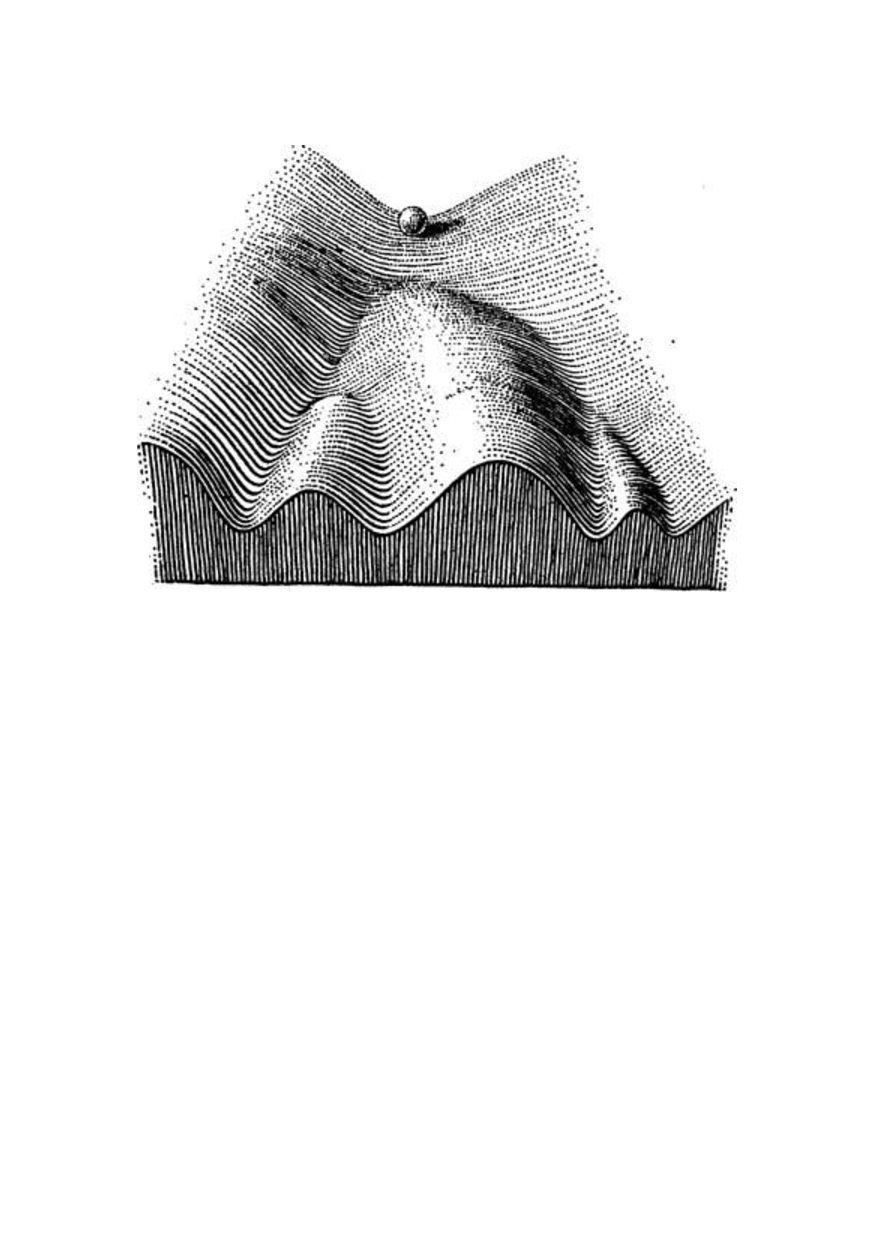
\includegraphics[width=8.45cm, height=\textheight, keepaspectratio]{{thesis_intro/figures/waddington_1957_chap2_fig4}.pdf}
    \end{center}
%    \tracingmacros=1
    \caption[The epigenetic landscape of a developing cell]{The epigenetic landscape of a developing cell, as envisioned by Waddington. The ball represents a cell at the beginning of development. Eventually the ball/cell will reach the bottom of the hill, ending up in one of several possible terminal cell types. The steep terrain counteracts most perturbations by forcing the ball back onto the path, making the whole process robust. Reprinted from Waddington, 1957\supercite{Waddington:1957ub}.}
%    \tracingmacros=0
    \label{fig:waddington_landscape}
\end{figure}
\clearpage

\begin{figure}[h]
    \begin{center}
    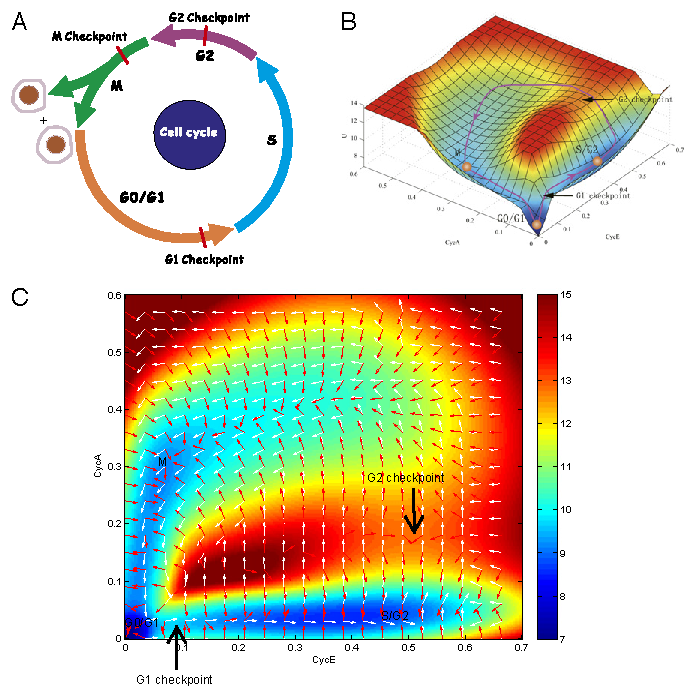
\includegraphics[width=8.45cm, height=\textheight, keepaspectratio]{{thesis_intro/figures/wang_2014_fig2}.pdf}
    \end{center}
    \caption[Three views of the mammalian cell cycle]{Three views of the mammalian cell cycle. A) The classical schematic view. B) The potential surface of the cell cycle. Data was taken from a 44 dimensional model and projected onto the concentrations of two cyclins, $CycA$ and $CycE$ (arbitrary units). The low points on the surface correspond to the various phenotypes along the cell cycle, and the transition path between them is shown. C) A 2D rendition of the complete epigenetic landscape of the model shown in B. The red arrows show the gradient of the potential, whereas the white arrows show the probability flux. Note that they never exactly coincide. Reprinted from Li et al., 2014\supercite{Li:2014iw}.}
    \label{fig:wang_cell_cycle_landscape}
\end{figure}
\clearpage

\begin{figure}[h]
    \begin{center}
    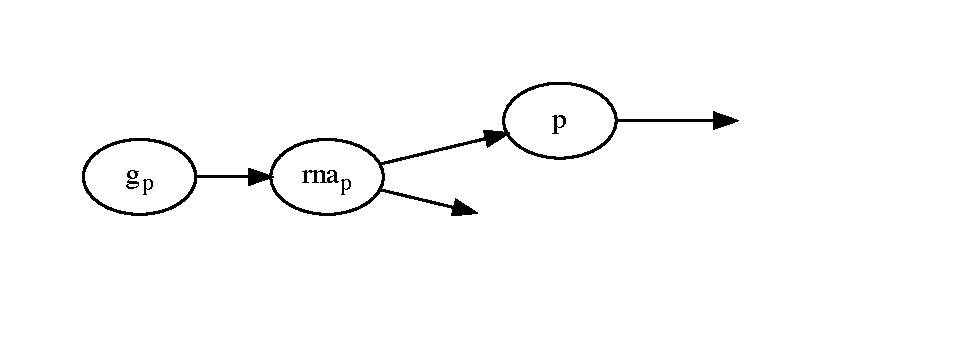
\includegraphics[keepaspectratio]{{thesis_intro/figures/simple_expression_digraph}.pdf}
    \end{center}
    \caption[A simple digraph representation of the simple gene expression model]{A simple digraph representation of the simple gene expression model from \eqref{eq:simple_expression}. An arrow from one species to another implies that the first species is involved in the production of the second. Arrows to empty space imply a decay reaction.}
    \label{fig:simple_expression_digraph}
\end{figure}
\clearpage

\begin{figure}[h]
    \begin{center}
    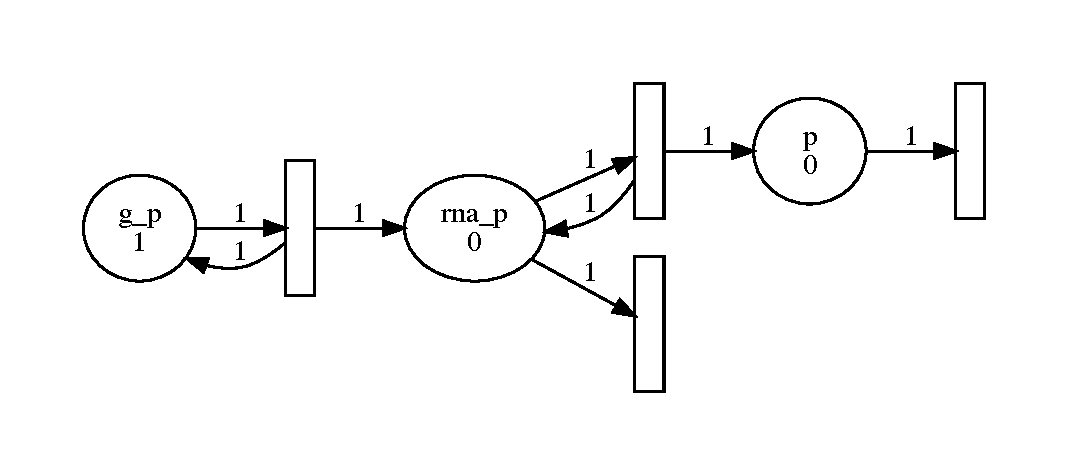
\includegraphics[width=1\textwidth,center]{{thesis_intro/figures/simple_expression_petri_net}.pdf}
    \end{center}
    \caption[A petri net representation of the simple genetic expression model]{A petri net representation of the simple genetic expression model from \eqref{eq:simple_expression}. Arrows starting at places (round nodes) and ending at transitions (rectangular nodes) imply that the connected species is a reactant in the connected reaction. Arrows starting at transitions and ending at places imply that the connected reaction produces the connected species. Above each arrow is a weight that gives its stoichiometry. The marking (the count of each species) is shown underneath the name of each species. Transitions that have no arrows leaving them imply a decay reaction.}
    \label{fig:simple_expression_petri_net}
\end{figure}
\clearpage

\begin{figure}[h]
    \begin{center}
    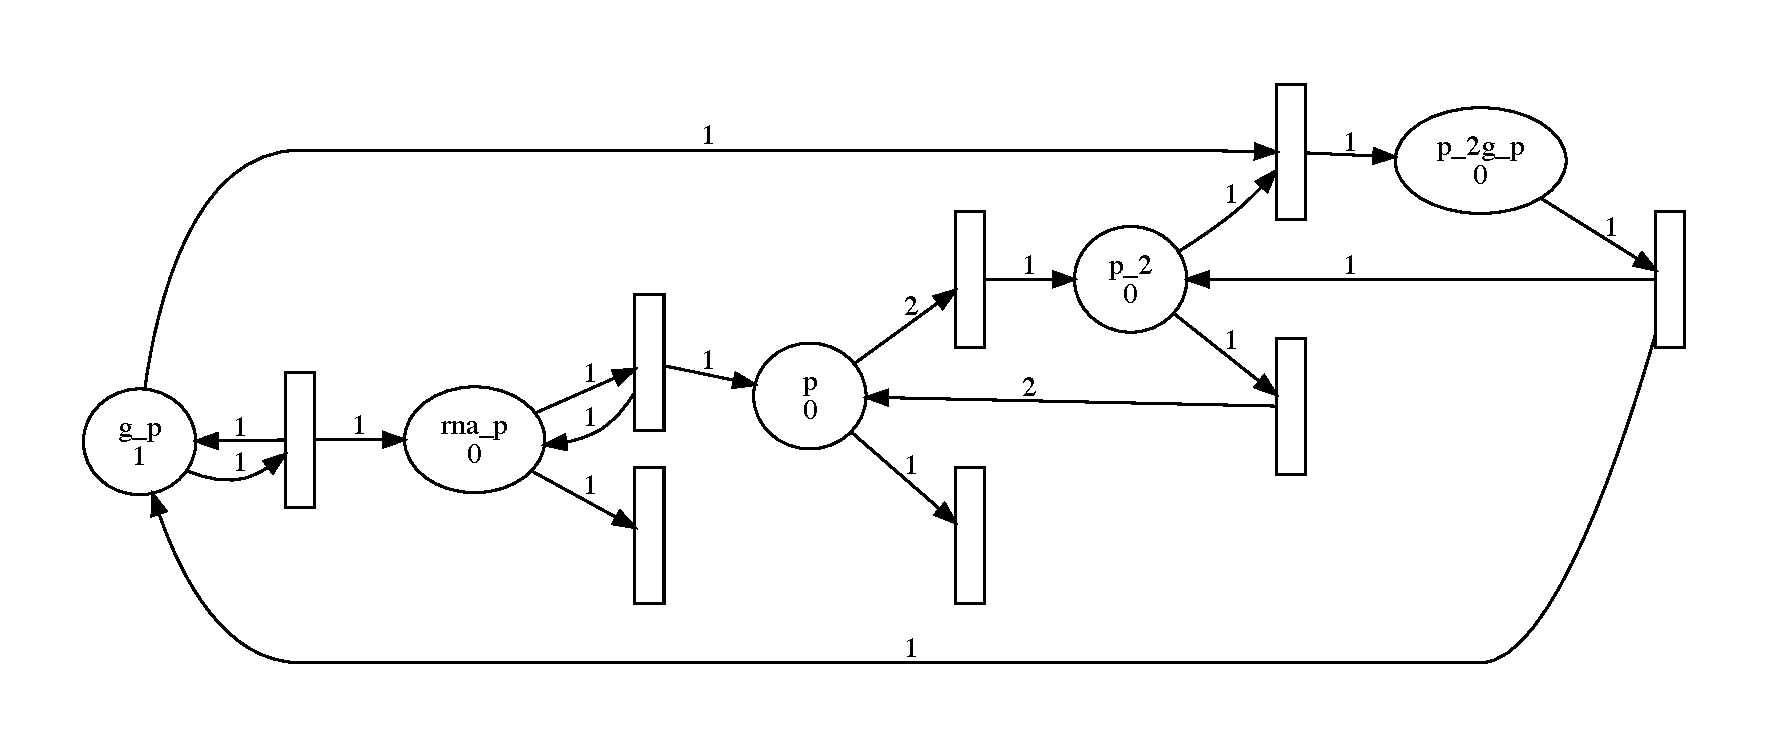
\includegraphics[width=1.2\textwidth,center]{{thesis_intro/figures/self_regulating_expression_petri_net}.pdf}
    \end{center}
    \caption[A petri net representation of the self regulating genetic expression model]{A petri net representation of the self regulating genetic expression model from \eqref{eq:self_regulating_expression}. The network is represented as described in \figref{fig:simple_expression_petri_net}.}
    \label{fig:self_regulating_expression_petri_net}
\end{figure}
\clearpage

\begin{figure}[h]
    \begin{center}
    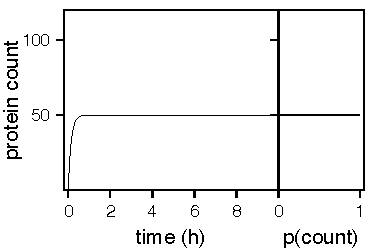
\includegraphics[keepaspectratio]{{thesis_intro/figures/simple_expression_timeseries_deterministic}.pdf}
    \end{center}
    \caption[Time series from a deterministic simulation of the simple expression system]{Time series from a deterministic simulation of the simple expression system (see \eqref{eq:simple_expression}) with ${ \condetx{1}=.1, \condetx{2}=.1, \condetx{3}=.1, \condetx{4}=2 \cdot 10^{-3} }$. The subplot along the left side shows the epigenetic landscape (as calculated via a histogram of the adjacent time series).}
    \label{fig:simple_expression_timeseries_deterministic}
\end{figure}
\clearpage

\begin{figure}[h]
    \begin{center}
    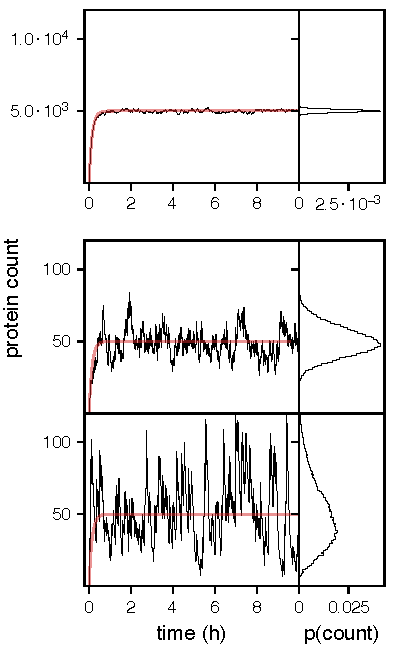
\includegraphics[keepaspectratio]{{thesis_intro/figures/simple_expression_timeseries_stochastic}.pdf}
    \end{center}
    \caption[Time series from stochastic simulations of the simple expression system]{(Black lines) time series from stochastic simulations of the simple expression system (see \eqref{eq:simple_expression}). The subplots along the left side show the epigenetic landscape of each variant (as calculated via a histogram of data from 10 simulation days, including the adjacent stochastic time series). (Red lines) the deterministic simulation of the same system, for comparison purposes. (Top panel) simple expression system with ${ \condetx{1}=10, \condetx{2}=.1, \condetx{3}=.1, \condetx{4}=2 \cdot 10^{-3} }$ (Middle panel) same, with ${ \condetx{1}=.1, \condetx{2}=.1, \condetx{3}=.1, \condetx{4}=2 \cdot 10^{-3} }$. (Bottom panel) same, with ${ \condetx{1}=.01, \condetx{2}=1, \condetx{3}=.1, \condetx{4}=2 \cdot 10^{-3} }$. The same constants were used in the deterministic and stochastic simulations (\ie $\constoch = \condet$). The mean expression level of the system simulated in the top panel is 100x that of the systems in the bottom two panels. From top to bottom the noise strengths are 1.98, 1.98, and 10.8039 (see \eqref{eq:simple_expression_noise_strength}).}
    \label{fig:simple_expression_timeseries_stochastic}
\end{figure}
\clearpage

\begin{figure}[h]
    \begin{center}
    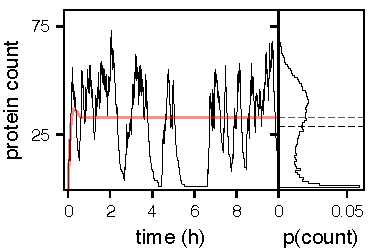
\includegraphics[keepaspectratio]{{thesis_intro/figures/self_regulating_expression_timeseries_stochastic}.pdf}
    \end{center}
    \caption[Time series from a stochastic simulation of the self regulating expression system]{(Black line) time series from a stochastic simulation of the self regulating expression system (see \eqref{eq:self_regulating_expression}). (Red line) the deterministic simulation of the same system. The subplot along the left side shows the epigenetic landscape. (Black and red dashed lines)  the mean protein expression value as calculated by stochastic and deterministic simulation, at $28.7$ and $33.0$ respectively ($15\%$ divergence). The deterministic rate constants used were ${ \condetx{1}=.1, \condetx{2}=.1, \condetx{3}=.1, \condetx{4}=2 \cdot 10^{-3}, \condetx{5}=10^{-6}, \condetx{6}=1, \condetx{7}=1, \condetx{8}=2 \cdot 10^{-3} }$. The stochastic rate constants were the same (\ie $\constoch = \condet$), except for $\constochx{5} = 2 \cdot \condetx{5} = 2 \cdot 10^{-6}$ (as per \eqref{eq:deterministic_second_order_self}).}
    \label{fig:self_regulating_expression_timeseries_stochastic}
\end{figure}
\clearpage

%\begin{figure}[h]
%    \begin{center}
%    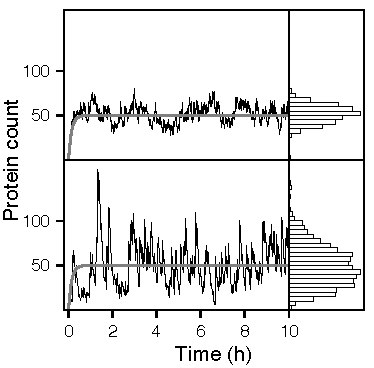
\includegraphics[keepaspectratio]{{thesis_intro/figures/simple_expression_timeseries_fixed_mean}.pdf}
%    \end{center}
%    \caption{(Black lines) time series from stochastic simulations of the simple expression system (see \eqref{eq:simple_expression}). The subplots along the left side show the epigenetic landscape of each variant (as calculated via a histogram of the stochastic time series). (Gray lines) the determistic simulation of the same system, for comparison purposes. (Top panel) simple expression system with ${ \condetx{1}=.1, \condetx{2}=.1, \condetx{3}=.1, \condetx{4}=.002 }$. (Bottom panel) same with ${ \condetx{1}=.01, \condetx{2}=1, \condetx{3}=.1, \condetx{4}=.002 }$. To first order, the noise scales\supercite{Ozbudak:2002iq} as $1 + \frac{\condetx{2}}{\condetx{3} + \condetx{4}}$.}
%    \label{fig:simple_expression_timeseries_fixed_mean}
%\end{figure}
%\clearpage

\begin{figure}[h]
    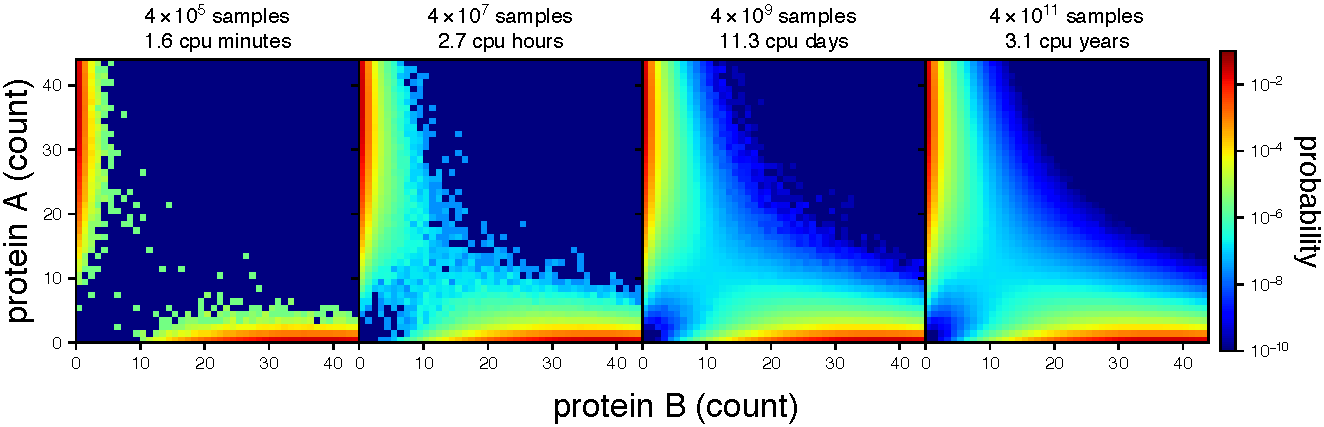
\includegraphics[width=1.2\textwidth,center]{{thesis_intro/figures/gts_theta_1en1_landscape_2d_comparison_samples}.pdf}
    \caption[Two dimensional epigenetic landscapes generated from the $\GTSSLOWEST$ system]{Two dimensional epigenetic landscapes generated from the $\GTSSLOWEST$ system (described in \secref{sec:gts}\todo{format in ECES paper so the preceeding secref works}). From left to right, the subplots show versions of the same landscape calculated using an increasing number of species count samples. The total sample count used in each landscape, and the CPU time used to collect those samples, is shown above each subplot. The samples were taken from 20 trajectories, each of which was generated using several thousand CPU cores running a parallelized implementation of \abr{SSA}\supercite{Roberts:2013cu}.}
    \label{fig:gts_theta_1en1_landscape_2d_comparison_samples}
\end{figure}
\clearpage

%\begin{figure}[h]
%    \begin{center}
%    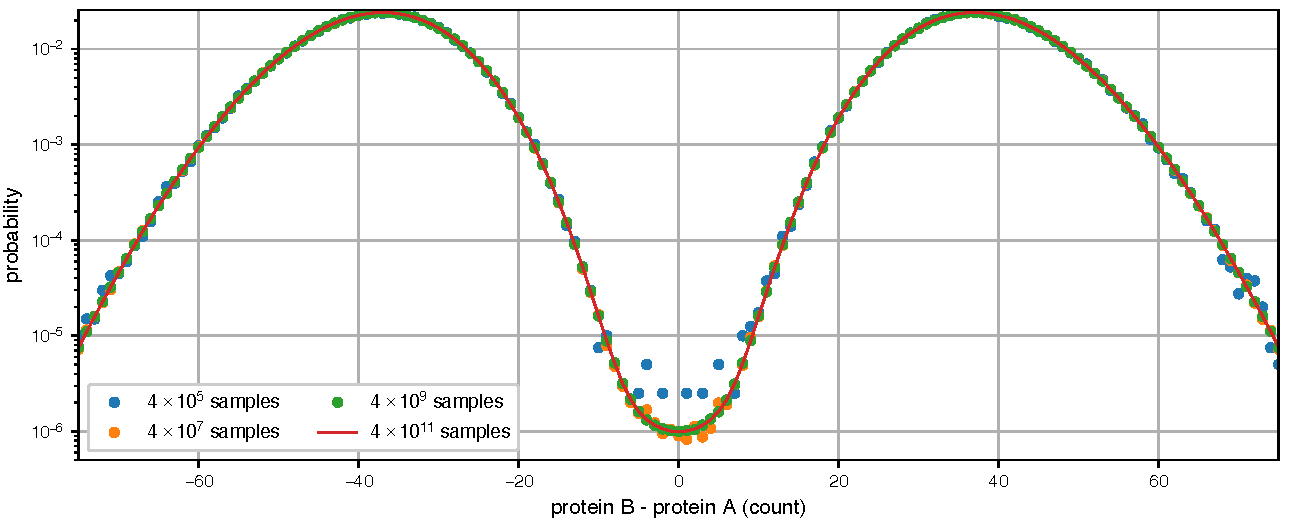
\includegraphics[width=1.2\textwidth,center]{{thesis_intro/figures/gts_theta_1en1_landscape_1d_comparison_samples}.pdf}
%    \end{center}
%    \caption{One dimensional versions of the two dimensional landscapes shown in \figref{fig:gts_theta_1en1_landscape_2d_comparison_samples}, shown overlapping for ease of comparison. The largest divergence between the landscapes calculated with different sample counts can be seen in the middle of the transition region, at $x=0$.}
%    \label{fig:gts_theta_1en1_landscape_1d_comparison_samples}
%\end{figure}
%\clearpage

\begin{figure}[h]
    \begin{center}
    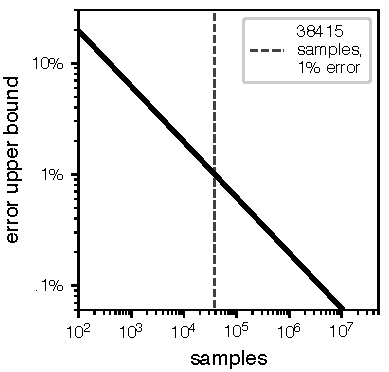
\includegraphics[keepaspectratio]{{thesis_intro/figures/sampling_error_mean_of_exponential}.pdf}
    \end{center}
    \caption[The margin of error vs sample count when using stochastic simulation to calculate the \abr{MFPT} of a rare state switching event]{The margin of error ($95\%$ confidence) vs sample count when using stochastic simulation to calculate the \abr{MFPT} of a rare state switching event. The x-axis begins at $100$ in order to emphasize that the relationship is only valid in the limit of large sample size. See \secref{sec:moe_from_simulation_params} for derivation and details.}
    \label{fig:sampling_error_mean_of_exponential}
\end{figure}
\clearpage

\begin{figure}[h]
    \begin{center}
    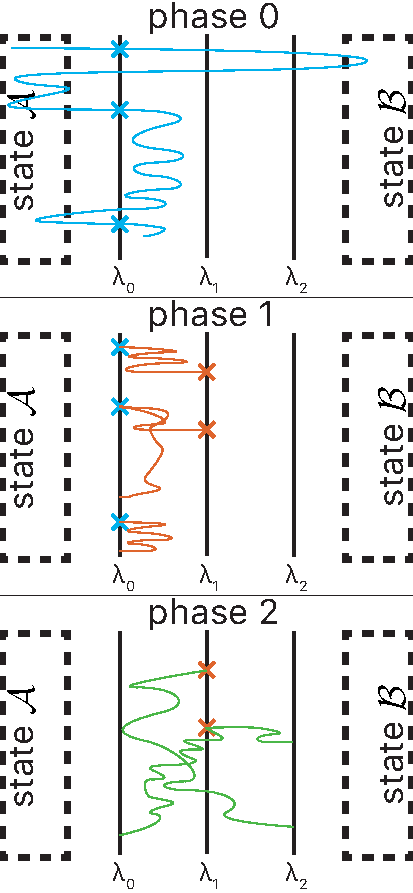
\includegraphics[keepaspectratio]{{thesis_intro/figures/fflux_stages}.pdf}
    \end{center}
    \caption[A schematic representation of a forward flux sampling (FFS) simulation]{A schematic representation of an \abr{FFS} simulation run from $\atob$. The simulation shown has 3 phases, one for each interface $\ifacei$ that is defined.\todo{maybe?: explain that simulation time increases towards the bottom of the y-axis on each subplot} During each phase $\phasegz$, trajectories are initialized from one of the points (chosen at random) where a trajectory in the previous phase crossed $\ifaceimo$ while traveling in the forward direction (\ie towards $\stateb$). During phase $2$ (the final phase), trajectories that cross $\ifacex{2}$ are considered to have completed the transition into $\stateb$.}
    \label{fig:fflux_stages}
\end{figure}
\clearpage

\begin{figure}[h]
    \begin{center}
    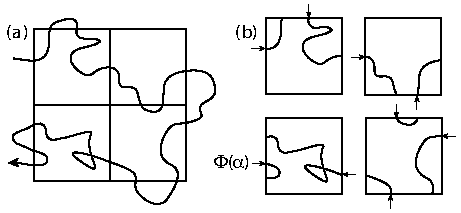
\includegraphics[keepaspectratio]{{thesis_intro/figures/dickson_2009_fig2}.pdf}
    \end{center}
    \caption[A simple schematic of a nonequilibrium umbrella sampling (NEUS) simulation]{A simple schematic of a nonequilibrium umbrella sampling (NEUS) simulation. A state space divided into 4 regions along a 2D order parameter is shown. \textbf{a)} An example of a single unconstrained stochastic trajectory run over the regions and the surrounding area. \textbf{b)} An example of several \abr{NEUS} trajectories constrained in each of the regions. When a trajectory leaves its starting region it is terminated, and a new trajectory is initialized at a state $\alpha$ within the same region. The choice of $\alpha$ is determined by the distribution of fluxes $\fluxx{\alpha}$ into each $\alpha$. Reprinted from Dickson et al., 2004\supercite{Dickson:2009gt}.}
    \label{fig:dickson_2009_fig2}
\end{figure}
\clearpage

\begin{figure}[h]
    \begin{center}
    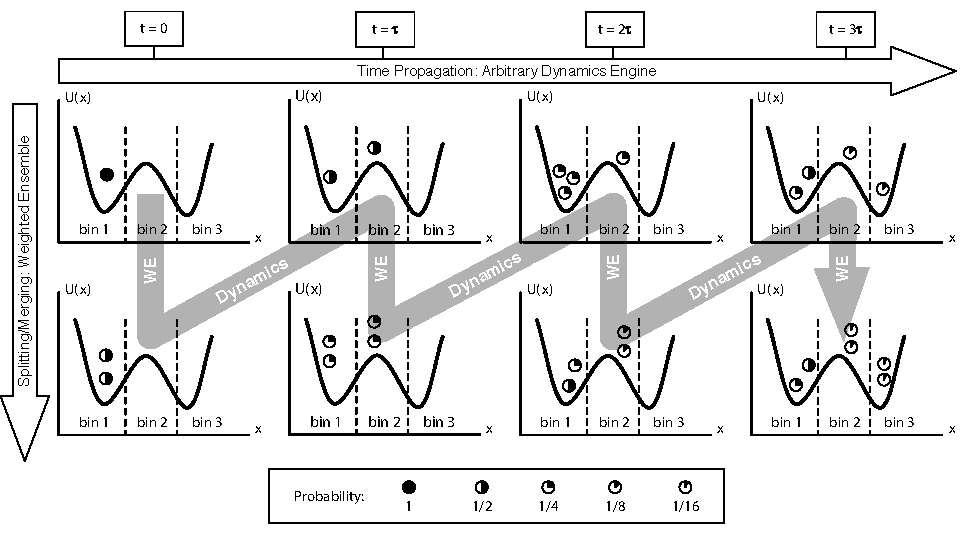
\includegraphics[width=1\textwidth,center]{{thesis_intro/figures/donovan_2013_fig1}.pdf}
    \end{center}
    \caption[An explainer schematic demonstrating the inner workings of weighted ensemble (WE) simulation]{An explainer schematic demonstrating the inner workings of weighted ensemble (WE) simulation. Reprinted from Donovan et al., 2013\supercite{Donovan:2013gz}.}
    \label{fig:donovan_2013_fig1}
\end{figure}
\clearpage

\end{subappendices}


\cleardoublepage
%\printbibliography[title={References}]
%\end{refsection}

%% If using Overleaf, you'll have to upload the resulting tex file & figures
%% since Overleaf does not support Rnw files right now (April 13, 2016)
%\begin{refsection}[rnw_chapter/rnw_chapter.bib]
%\include{rnw_chapter/rnw_chapter}
%\cleardoublepage
%\printbibliography[title={References}]
%\end{refsection}
%
%\begin{refsection}[conclusion_chapter/conclusion_chapter.bib]
%\chapter{Discussion and conclusion}
\label{chap:conclusion}

The epigenetic landscapes of complex genetic regulation networks can be mapped using stochastic simulation. The presence of rare events in these regulatory networks makes the traditional stochastic methods non-practical (in terms of computation time). Our theoretical analysis shows for the first time that a complete \abr{FFS} simulation, including phase $0$, can indeed be used to significantly speed up stochastic simulation of complex systems with rare events. We also show that there are significant sources of error in the \abr{FFS} approach that have not been fully considered by the existing analyses.

The \abr{FFPilot} method is an enhanced sampling method that controls error in an optimal way. For simulations of simple enough systems, this error control is exact and precise. For any system with a 1D landscape, \abr{FFPilot} will produce results with a consistent, predictable, user-set upper bound on the margin of error. For multi-dimensional systems without rough landscapes, error is still controlled, but not precisely. For these more complex systems there is an anomalous extra error that is not fully accounted for by the theory and algorithms that drive \abr{FFPilot}. The reasons why are complicated, but can be summarized with one word: covariance. We established that correlations between the sets of states used in each phase to launch new trajectories are sufficient to explain the anomalous error.

It is possible to perform an alternative derivation of the simulation variance that takes the phase-by-phase covariance into account. Instead of zeroing out the covariances in \eqref{eq:PWest_variance_expansion}, they can be left as-is. This will end up giving what is effectively an extra term in the definition of the margin of error given in \eqref{eq:product_estimator_zeta}:
\begin{align*}
    \moefunc{\PWest} &= \zscore \sqrt{\sum_i \sum_j \frac{\sigma_{ij}}{\pwtruex{i} \pwtruex{j} \sqrt{n_i} \sqrt{n_j}}}, \\
    \moefunc{\PWest} &= \zscore \sqrt{\sum_i \frac{\pwvtrue}{\pwtruesq n_i} + \sum_i \sum_{j \neq i} \frac{\sigma_{ij}}{\pwtruex{i} \pwtruex{j} \sqrt{n_i} \sqrt{n_j}}}.
\end{align*}
Initial investigation suggests that a simple closed form equation that optimizes the run counts $n_i$ and $n_j$ (like \eqref{eq:optimizing_equation_general} or \eqref{eq:optimizing_equation_ffpilot}) cannot be found when the covariance term is included. However, it is still likely that a reasonable optimization scheme (probably involving some numerical minimization) can be developed. Additionally, it should be possible to estimate the phase-by-phase covariances $\sigma_{ij}$ using some variant of the scheme currently used by \abr{FFPilot} to estimate the phase zero variance $\pwvtruex{0}$. Thus, it is likely that an \abr{FFPilot} version 2 could be developed that would fully take the covariances into account.

In summary, we show that it is possible to get speedups on the order of 100x when simulating genetic regulatory networks by using enhanced sampling methods. As the enhanced sampling methods, and the theory behind them, are further refined, it should be possible to get the fullest possible speedup in a completely automated way, one that is no more complex to use than standard stochastic simulation methods.
%\cleardoublepage
%\printbibliography[title={References}]
%\end{refsection}


% CV PDF file downloaded from the moderncv template available at Overleaf
% https://www.overleaf.com/latex/templates/modern-cv-and-cover-letter-2015-version/sttkgjcysttn#.Vw6PFRMrL65
%\includepdf[pages={-}, pagecommand={\thispagestyle{plain}}]{moderncv-2015.pdf}


\newpage
\footnotesize
\bibliographystyle{unsrt}
\bibliography{bib/error_control_of_enhanced_sampling,bib/thesis_intro}

\end{document}
